
\section{Estimation of deterministic parameters: Large numbers law and sample estimators}
\subsection{The estimation problem and properties of an estimator}
\subsubsection{The estimation problem}
\begin{itemize}
    \item \textbf{Problem}:
     Given the observed signal \(x(t)\) for \(t\in[0,T)\), that is a realization of the random process \(X(t)\), we want to determine the value of a parameter \(\theta\) that is not directly observable but is related in same way to \(X(t)\), i.e. all the process realizations are affected by the value of \(\theta\), so also the particular realization we observe in \([0,T)\).
     \[
     \text{Observed signal: }X(t;\theta)\qquad t\in[0,T)
     \]
     \item \textbf{Mathematical model of the data:} The first step is to derive the mathematical model we are looking for, first we have to represent the continuous-time observed signal in discrete form(basis expansion).
     \item \textbf{Discrete representation of the obeserved signal}: to derive the mathematical model we are looking for, we have to represent the continuous-time observed signal in discrete form(basis expansion).
     \item Given the characteristics of the observed signal, we first determine a basis \(\mathbf{basis}\) \(\mathbf{\Psi}\) that allows to represent all possible realizations of process \(X(t)\), then we derive the corresponding image vector \textbf{X}.
     \item \textbf{Discrete representation of the observed signal:}
    \[ \text{Osberved signal:} \quad X(t; \theta) \quad t \in [0, T) \quad \overset{\Psi}{\Longleftrightarrow} \quad \mathbf{X}(\theta) \quad \text{image vector}\]
    \item \textbf{The data model:} being \(X(t)\) a random process, the image vector \(\textbf{X}\) is a random vector, so its statistical behavior is completely characterized by its joint probability density function (pdf):
    \[
    \text{Observed data in discrete form:} \quad \mathbf{X}(\theta) \quad \Rightarrow \quad f_X(\mathbf{x};\theta)
    \]
    \item \textbf{The estimation problem: } given the observed data vector \textbf{x},determine a measure (as much accurate as possible) of the unknown parameter \(\theta\):
    \[
\hat{\theta} = g(\mathbf{x})
\quad \Longrightarrow \quad
\text{The estimator is a function of the data vector } \mathbf{x}
\]
\[
\Longrightarrow \quad \hat{\theta} \text{ is a random variable (r.v.)}
\]
   \item \textbf{Discrete representation of the observed signal}:
   \[ \text{Osberved signal:} \quad X(t; \theta) \quad t \in [0, T) \quad \overset{\Psi}{\Longleftrightarrow} \quad \mathbf{X}(\theta) \quad \text{image vector}\]
   \item If the process \(X(t)\) has rigorously finite bandwidth \(B\) or ti has essential bandwidth \(B\) at level \(\alpha\), with \(N=2BT\gg1\), such that \(\alpha\ll1\), we can represent \(X(t)\) in discrete form by using the orthonormal basis of dimension \(N=2BT\) of sinc functions, i.e. the continuous-time observed signal is discretized by collecting \(N=2BT\) samples at time intervals multiples of \(T_c=1/2B\) within the observation interval \([0,T)\):
   \[
\mathbf{X} = \begin{bmatrix}
\mathbf{X}[0] & \mathbf{X}[1] & \cdots & \mathbf{X}[N-1]
\end{bmatrix}^T
= \frac{1}{\sqrt{2B}}
\begin{bmatrix}
X(0) & X(T_c) & \cdots & X((N-1)T_c)
\end{bmatrix}^T
\]\[
\text{Dimension of the image vector:} \quad N = \frac{T}{T_c} = 2BT
\]
\begin{figure}[H]
    \centering
    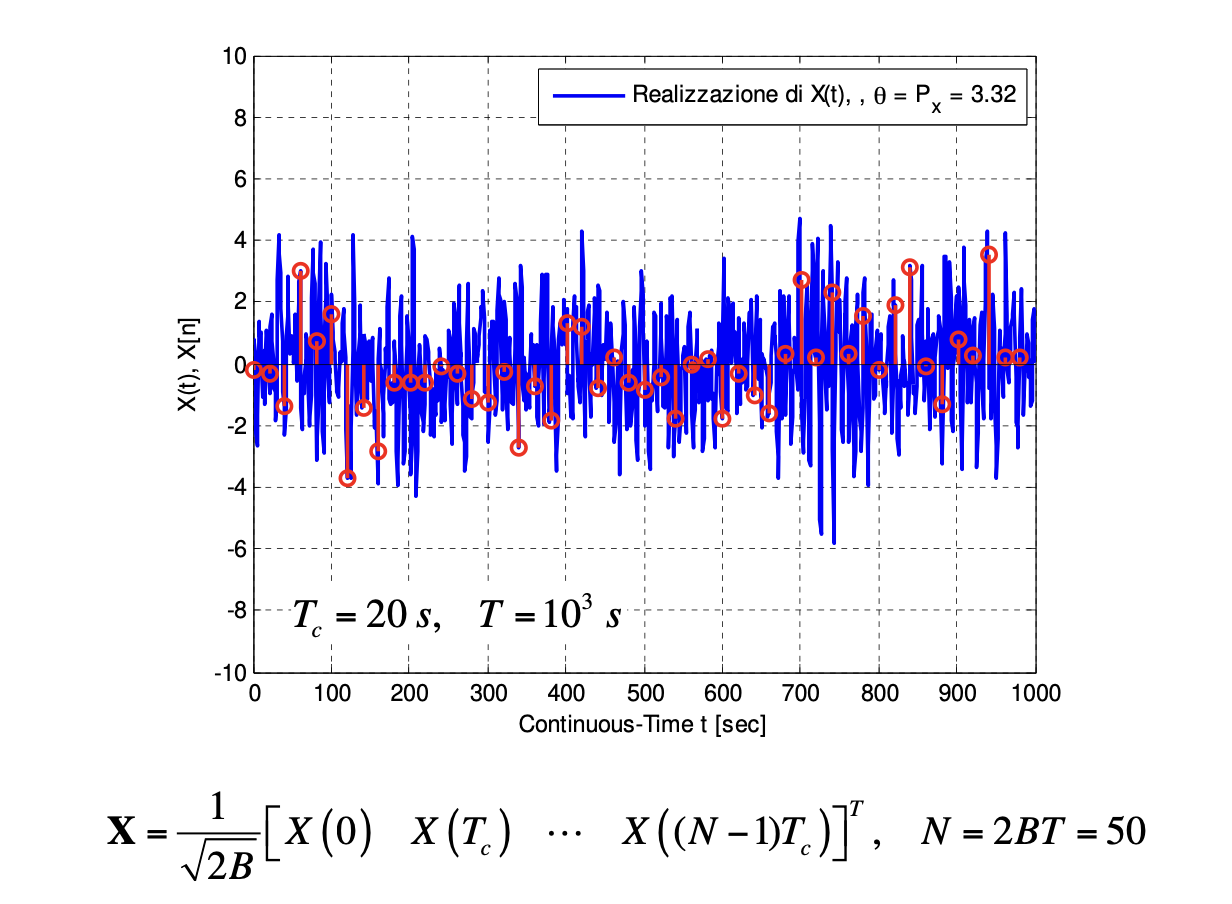
\includegraphics[width=0.75\linewidth]{Image/pdf 3/1.Estimation_problem.png}
    \label{fig:placeholder}
\end{figure}
\end{itemize}
\subsubsection{The properties of an estimator}
\begin{itemize}
    \item \textbf{Estimator:} \(\hat{\theta}=g(\textbf{x})\) is a function of the observed data vector \textbf{X}, hence it is a random variable.
    \item The full statistical characterization of the estimator is provided by its pdf.
    \item If we know the pdf of the data vector, we can derive the pdf of the estimator by applying the \textbf{fundamental theorem} for the trasformation of random variables or the method of the cumulative distribution function:
    \[
    \mathbf{X}(\theta)\Rightarrow f_X(\mathbf{X};\theta)\Rightarrow f_{\hat{\theta}}(\hat{\theta};\theta)
    \]
    \item The statistical behavior of the estimator depends on the entire pdf. However, it is common pratice to use as \textbf{quality index} of an estimator a specific moment of the pdf, that is calle \textbf{mean square error(MSE)} and represents the statistical power of the estimation error.
    \item Also, the mean value of the estimation error \textbf{bias} plays an important role.
    \item \textbf{Estimation error:}
    \[
    \varepsilon(\mathbf{x})\triangleq \theta-\hat{\theta}(\textbf{x})\longrightarrow \varepsilon\text{ is a random variable}
    \]
    \item \textbf{Mean square error(MSE)}, \textbf{variance} and \textbf{bias} of the estimate of a parameter \(\theta\) are mutually related. Assume that the parameter is \textbf{\underline{deterministic}}(we will analyze the case of random parameters separately):
    \[
MSE\{ \hat{\theta} \} \triangleq E \left\{ \left| \theta - \hat{\theta} \right|^2 \right\}, \quad
\text{var} \{ \hat{\theta} \} \triangleq E \left\{ \left| \hat{\theta} - E\{\hat{\theta}\} \right|^2 \right\}, \quad
b\{\hat{\theta}\} \triangleq E\{\theta - \hat{\theta}\}
\]

\[
MSE\{ \hat{\theta} \} = E \left\{ | \theta - \hat{\theta} |^2 \right\}
= \int_{-\infty}^{+\infty} | \theta - \hat{\theta} |^2 f_{\hat{\theta}}(\hat{\theta}; \theta) d\hat{\theta}
= \int \! \!\! \int | \theta - \hat{\theta}(\mathbf{x}) |^2 f_X(\mathbf{x}; \theta) d\mathbf{x}
\]
    \item Note that in general the MSE depends on the value of \(\theta\)
    \item \textbf{Bias} and \textbf{MSE} of an estimator are the first and second order moments of the estimation error, which is a random variable:
    \[
\text{Estimation error: } \varepsilon(\mathbf{x}) \triangleq \theta - \hat{\theta}(\mathbf{x}) \quad
{\Longrightarrow}\quad
\begin{cases}
b\{\hat{\theta}\} \triangleq E\{\varepsilon\} = E\{\theta - \hat{\theta}\} = \theta - E\{\hat{\theta}\} \\
\\
MSE\{\hat{\theta}\} \triangleq E\{|\varepsilon|^2\} = E\left\{|\theta - \hat{\theta}|^2\right\}
\end{cases}
\]
\item \textbf{MSE,variance} and \textbf{bias} of the estimate of \(\theta\) are related as follows:
\[
MSE\{ \hat{\theta} \} = E \left\{ | \theta - \hat{\theta} |^2 \right\}
= E \left\{ \left| \theta - E\{\hat{\theta}\} + E\{\hat{\theta}\} - \hat{\theta} \right|^2 \right\}
\]
\[
= E\left\{ \left| \theta - E\{\hat{\theta}\} \right|^2 \right\}
+ E\left\{ \left| E\{\hat{\theta}\} - \hat{\theta} \right|^2 \right\}
+ 2 E\left\{ \left( \theta - E\{\hat{\theta}\} \right) \left( E\{\hat{\theta}\} - \hat{\theta} \right) \right\}
\]
\[
= |\theta - E\{\hat{\theta}\}|^2
+ E\left\{ | E\{\hat{\theta}\} - \hat{\theta}|^2 \right\}
= b\{\hat{\theta}\}^2
+ \text{var}\{ \hat{\theta} \}
\]
\[
MSE\{\hat{\theta}\}=|b\{\hat{\theta}\}|^2+\text{var}\{\hat{\theta}\}
\]
\item The MSE(statistical power of the estimation error) can be reduced by reducing the bias (mean value of the estimation error) and/or by reducing the error variance (the variance is a measure of dispersion of a r.v. around its mean value).
\item An estimator that is \underline{unbiased} and has the \underline{minimum variance} is called \textbf{Minimum variance unbiased(MVU)} estimator.
\item An estimator of \(\theta\) that has MSE lower than another estimator of \(\theta\) is said to be more \textbf{efficient} than the other.
\item \textbf{Questions}: Does it exist an estimator that is the \textbf{most efficient}, i.e. an estimator having the \textbf{lowest MSE}? The answer is NO if we are talking about deterministic parameters. Whereas, the answer is YES for random parameters.
\item Any estimator of the unknown parameter \(\theta\) is a function of the observed data vector \textbf{x} and so also of the data size \(N\). If we want to stress this dependecy we can add the subscript \(N\):
\[
\hat{\theta}_N\equiv\hat{\theta}_N(\textbf{x})
\]
\item An estimator is \textbf{unbiased} if the mean value of the estimator is equal to the true value of the parameter, i.e. \underline{if the error is zero mean}.
\item If instead the mean value of the error is different from zero, it is called \textbf{bias} and the estimator \textbf{biased}.
\[
\text{Bias: } \quad b\{\hat{\theta}_N(\mathbf{x})\} \triangleq E\{\varepsilon_N(\mathbf{x})\}
= E\{\theta - \hat{\theta}_N(\mathbf{x})\}
= \theta - E\{\hat{\theta}_N(\mathbf{x})\}
\]
\[
\text{Unbiased estimator:} \quad b\{\hat{\theta}_N(\mathbf{x})\} = 0
\Longrightarrow E\{\hat{\theta}_N(\mathbf{x})\} = \theta
\]\[
\text{Biased estimator:} \quad b\{\hat{\theta}_N(\mathbf{x})\} \neq 0
\Longrightarrow E\{\hat{\theta}_N(\mathbf{x})\} \neq \theta
\]
\item An estimator is \textbf{asymptotically unbiased} if the bias goes to zero when the data size \(N\) grows to infinity:


\item An estimator is \textbf{consistent} if the estimate converges \textbf{in probability} of the true value of the parameter when the data size \(N\) grows to infinity:
\[
\lim_{N \to \infty} \Pr \left\{ \left| \hat{\theta}_N(\mathbf{x}) - \theta \right| \geq \varepsilon \right\} = 0
\quad \forall\, \varepsilon > 0
\]
\item Usually, it is not easy to verify the \textbf{convergence in probability} of an estimator. It is easier to verify the \textbf{mean square convergence}: this kind of convergence is guaranteed when the estimator is asymptotically unbiased and the estimate variance goes to zero when the data size \(N\) grows to infinity.
\item An estimator converges in \textbf{mean square sense(m.s.s.)} to the true value of the parameter if:
\[
\lim_{N \to \infty} E\left\{ \left| \hat{\theta}_N(\mathbf{x}) - \theta \right|^2 \right\}
= \lim_{N \to \infty} MSE\left\{ \hat{\theta}_N(\mathbf{x}) \right\} = 0
\]
\item Now, since it holds a true that:

\(\longrightarrow\) \textbf{convergence in mean square sense} is guaranteed when the estimator is asymptotically unbiased and the estimation variance goes to zero when the data size \(N\) grows to infinity, as previously stated.
\item \underline{If an estimator converges in mean square sense, it also converges in probability.} The reverse is not true, i.e. convergence in probability does not imply mean square convergence.
\item \textit{PROOF}. If we apply the \textbf{Bienaymè-Tchebycheff inequality}: 
\[
X \equiv \hat{\theta}_N
\quad
a \equiv \theta
\]
\[
\Pr \{ | X - a | \geq \varepsilon \} \leq \frac{ E \left\{ | X - a |^2 \right\} }{ \varepsilon^2 }
\]
\[
\lim_{N \to \infty} \Pr \{ | \hat{\theta}_N - \theta | \geq \varepsilon \} \leq \frac{ \lim_{N \to \infty} E \left\{ | \hat{\theta}_N - \theta |^2 \right\} }{ \varepsilon^2 } = 0
\]
\item Since the limit on the left-hand side cannot be negative, it must necessarily be zero, so mean square convergence implies convergence in probability.
\end{itemize}
\subsection{Taxonomy of the estimation problems}
\begin{itemize}
    \item The first distintion is between \textbf{deterministic parameters} and \textbf{random parameters}:
    \textbf{Deterministic parameters:}
\begin{itemize}
    \item probability of an event $p = \Pr\left\{A\right\}$
    \item moments of a distribution (mean value, variance, skewness, kurtosis, \textit{etc.})
    \item parameters of a distribution
    \item parameters of a signal (amplitude, phase, frequency, time of arrival, \textit{etc.})
    \item moments of a random vector (mean vector, correlation matrix, \textit{etc.})
    \item moments of a random signal (mean value function, ACF, PSD, \textit{etc.})
\end{itemize}
ACF=Autocorrelation Function,\quad PSD=Power Spectral Density

\textbf{Random parameters:}
\begin{itemize}
    \item parameters of a signal of which we know the a-priori pdf
    \item random signals (values of a realization of a random process)
\end{itemize}
\item According o the class to which the parameter/signal belongs to, different methods have been developed. We will investigate the principal ones:
\textbf{Deterministic parameters:}
\begin{itemize}
    \item Sample estimates (application of the Law of large numbers)
    \item Method of Moments (MM)
    \item Maximum Likelihood (ML) method
    \item Least Squares (LS): Linear LS or Non Linear LS (NLLS)
\end{itemize}

\textbf{Random parameters:}
\begin{itemize}
    \item Bayesian estimators (MMSE, LMMSE, MAP)
    \item LMMSE (for filtering/smoothing/prediction of random signals)
\end{itemize}

MMSE = Minimum Mean Square\\
LMMSE = Linear Minimum Mean square Error\\
MAP = Maximum A Posteriori
\end{itemize}
\subsection{Large Numbers Law and Measure of the Probability of an Event}
\subsubsection{Measure of the Probability of an Event}
\begin{itemize}
    \item A \textbf{Random experiment} is a process by which we observe something uncertain. After the experiment, the result of the random experiment is known.
    \item An \textbf{outcome} is a result of a random experiment. The set \(\Omega\) of all possible outcomes is called the \textbf{sample space}. Thus, in the context of a random experiment, the sample space \(\Omega\) is our universal set.
    \item Some \underline{examples} of random experiments and their sample spaces:
    \begin{itemize}
        \item toss a coin; sample space: \(\Omega=\{H,T\}\)(heads, tails)
        \item roll a die; sample space: \(\Omega=\{1,2,3,4,5,6\}\)
        \item observe the number of iPhones sold by an Apple store in Pisa in 2018; sample space: \(\Omega=\{0,1,2,3,\cdots\}\)
    \end{itemize}
    \item When we repeat a random experiment several times, we call each one of them a \textbf{trial}. Thus, a trial is a particular performance of a random experiment. Note that the sample space is defined based on how you define your random experiment.
    \item It is given a \textbf{random experiment} described by the triad \(S=(\Omega,F,P)\), where:
        \begin{itemize}
            \item \(\Omega \) = sample space(union of all elementary outcomes)
            \item \(F\) = set of all events (all possible outcomes and unions of them)
            \item \(P\) = probability map (it associates a probability to any event in F)
        \end{itemize}
    \item Assume we are interested on a particular event \(A\in F\), which as \textbf{probability of accurance} \(p\), i.e. \(Pr\{A\}=p\)
    \item \textbf{Problem:} we want to measure, i.e. estimate, the \underline{probability of occurence \(p\) of the event A} having the possibility to run the experiment \(N\) times under the same conditions and in such a way that the outcome of each trial is independent from the outcomes in the other trials.
    \item \textbf{Observed data} : they are given by the \(N\) outputs of the \(N\) trials of the random experiment. In particular, at the end of each trial, we observe if the event \(A\) occurs or not. Note that in this case \underline{the data are already in the discrete format}.
    \item Let us now define the following random variables (r.v.'s):
        \[
X_i \triangleq
\begin{cases}
0 & \text{if the event } A \text{ does not occur in the } i\text{-th trial} \\
1 & \text{if the event } A \text{ occurs in the } i\text{-th trial}
\end{cases}
\]

\[
K \triangleq \sum_{i=1}^{N} X_i \qquad \text{Number of times } A \text{ occurs over the } N \text{ trials}
\]
    \item The \(\{X_i\}\) are our observed data. They are binary random variables.
    \item Due to assumption that the \(N\) trials are run under the same conditions and each one independently from the others, we have that \(\{X_i\}\) are \textit{independent and identically distributed (IID)} random variables.
    \item As a consequence \(K\) is a \textbf{binomial} r.v. of parameters \(N\) and \(p\).
    \item \textbf{Mean value} and \textbf{variance} of the IID binary random variables \(\{X_i\}\).
    \[
X_i \triangleq
\begin{cases}
0 & \text{if the event } A \text{ does not occur in the } i\text{-th run} \\
1 & \text{if the event } A \text{ occurs in the } i\text{-th run}
\end{cases}
\]

\[
\Pr\{A\} = p \implies \Pr\{X_i = 1\} = \Pr\{A\} = p, \quad \Pr\{X_i = 0\} = \Pr\{\overline{A}\} = 1 - p
\]

\[
\text{Probability mass function (pmf):}
\]
\[
p_{X_i}(x) = \Pr\{X_i = x\} = (1-p)\delta[x] + p\delta[x-1], \quad \forall i
\]
\hspace{1cm} \text{(Kronecker's delta function)}

\[
\begin{cases}
\eta_X = E\{X_i\} = (1-p)\cdot0 + p\cdot1 = p \\
P_X = E\{X_i^2\} = (1-p)\cdot0^2 + p\cdot1^2 = p \\
\sigma_X^2 = \operatorname{var}\{X_i\} = E\left\{(X_i-\eta_X)^2\right\} = P_X - \eta_X^2 = p - p^2 = p(1-p)
\end{cases}
\]
    \item \textbf{Mean value} and \textbf{variance} of the binomial random variable \(K\):
    \[
K \triangleq \sum_{i=1}^{N} X_i \implies K \in \mathcal{B}(p, N)
\]

\[
\text{pmf:}
\]
\[
p_K(k) = P\{K = k\} = \binom{N}{k} p^{k} (1-p)^{N-k}, \quad 0 < p < 1,\quad 0 \leq k \leq N
\]

\[
\left\{
\begin{aligned}
    &\eta_K = m_K(1) = E\{K\} = \sum_{k=0}^{N} k\,p_K(k) = Np \\
    &\sigma^2_K = \mu_K(2) = \operatorname{var}\{K\} = E\{(K - \eta_K)^2\} = E\{K^2\} - \eta_K^2 \\
    &\phantom{\sigma^2_K} = \sum_{k=0}^{N} k^2\,p_K(k) - \eta_K^2 = Np(1-p)
\end{aligned}
\right.
\]
   \begin{figure}[H]
       \centering
       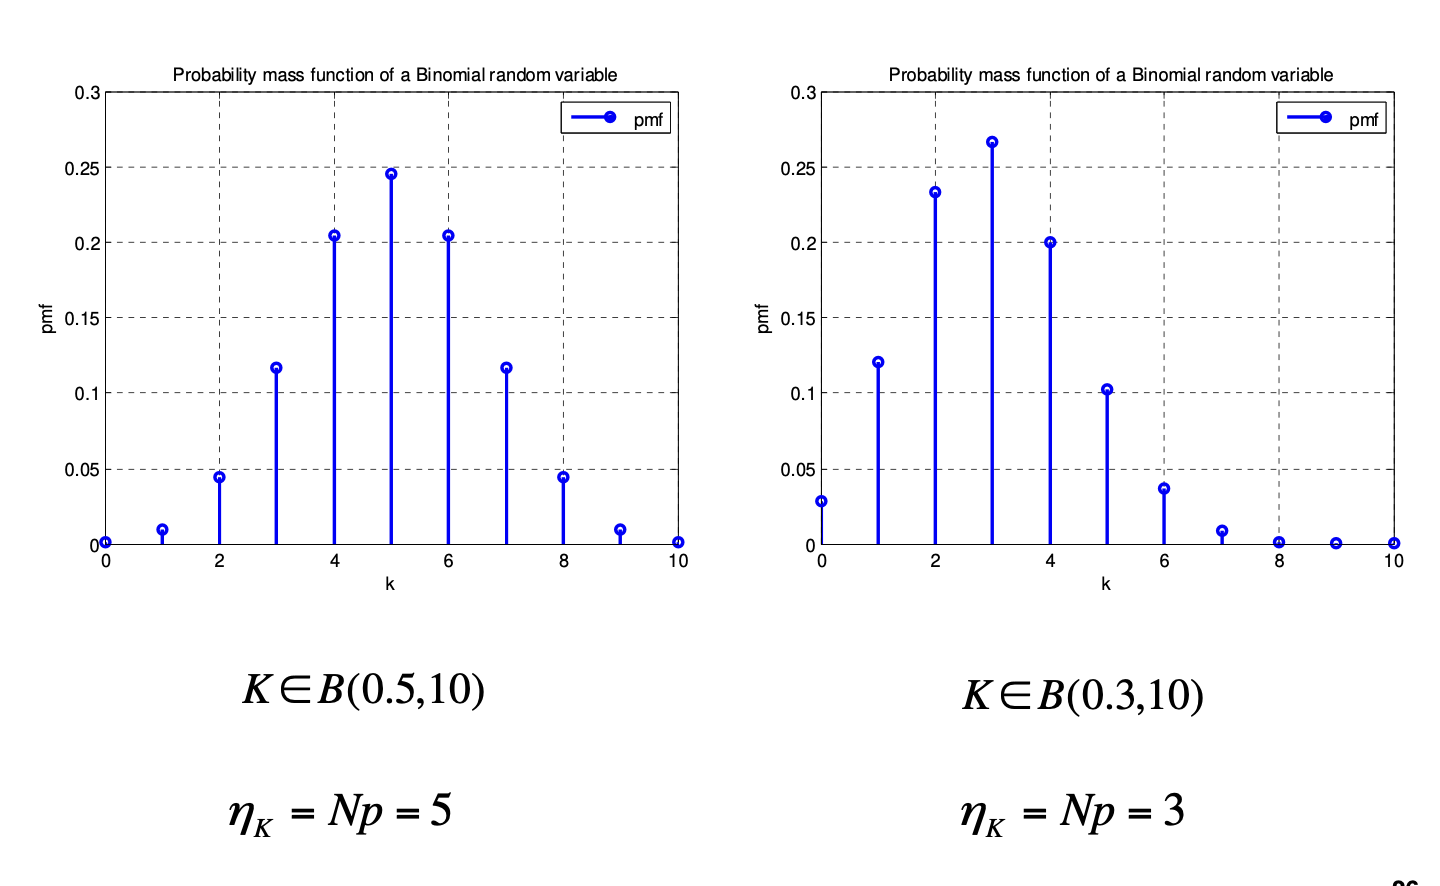
\includegraphics[width=0.75\linewidth]{Image/pdf 3/2.Prob_Event.png}
       \label{fig:placeholder}
   \end{figure}
   \begin{figure}[H]
       \centering
       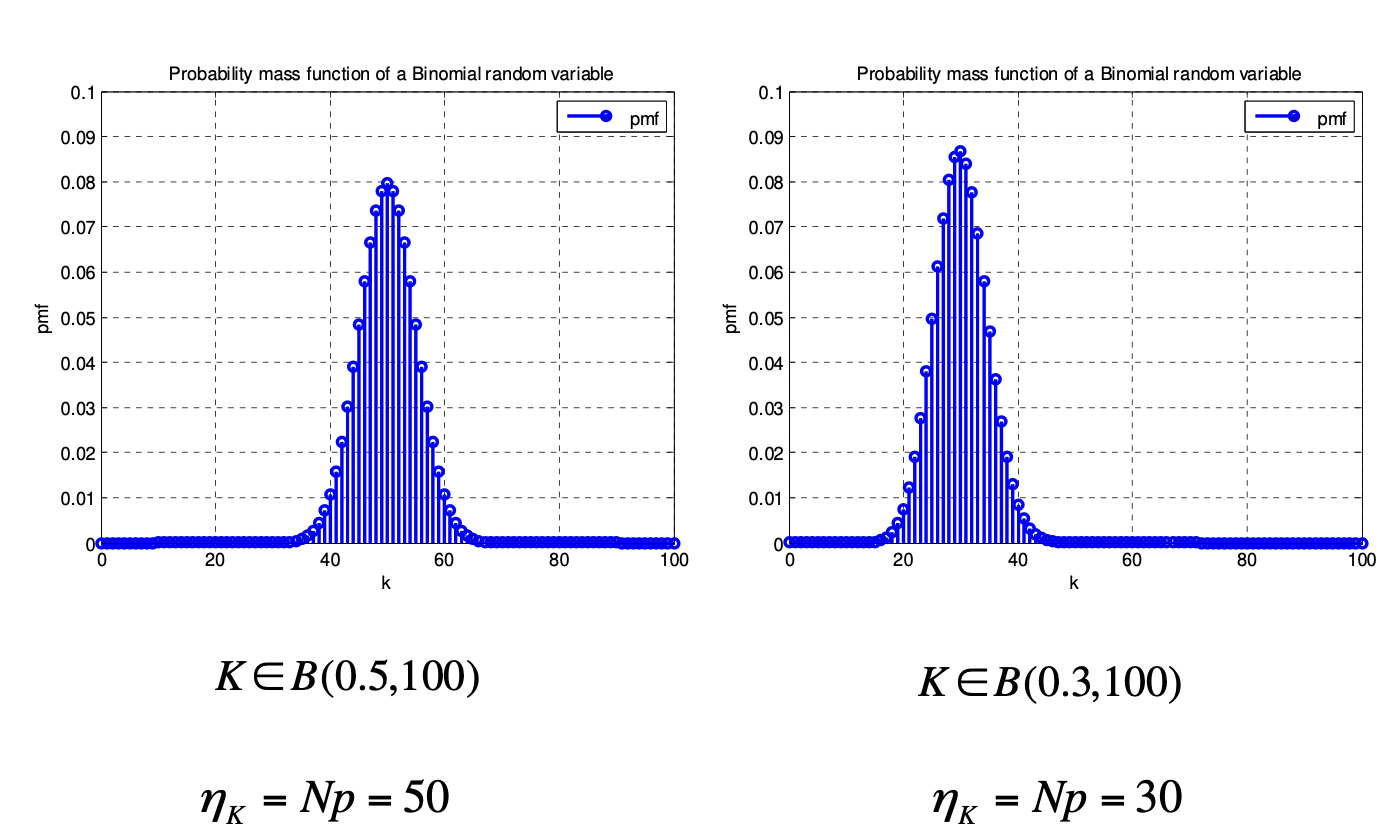
\includegraphics[width=0.75\linewidth]{Image/pdf 3/3.prob_event_2.png}
       \label{fig:placeholder}
   \end{figure}
   \item \textbf{Mean value} and \textbf{variance} of the binomial r.v. \(K\):
   \[
K \in \mathcal{B}(p, N)
\iff
K = \sum_{i=1}^{N} X_i, \quad X_i \in \{0, 1\}, \quad \Pr\{X_i = 1\} = p
\]

\[
\left\{
\begin{aligned}
    &\eta_X = E\{X_i\} = p \\
    &\sigma_X^2 = \operatorname{var}\{X_i\} = p(1-p)
\end{aligned}
\right.
\]

\[
\begin{aligned}
    \eta_K = E\{K\} &= E\left\{\sum_{i=1}^{N} X_i\right\}
    = \sum_{i=1}^{N} E\{X_i\}
    = \sum_{i=1}^{N} p
    = Np
\end{aligned}
\]
\[
\sigma_K^2 = \operatorname{var}\{K\} = E\{(K - Np)^2\} = E\left\{\left( \sum_{i=1}^N X_i - Np \right)^2 \right\}
\]

\[
= E\left\{ \left( \sum_{i=1}^N (X_i - p) \right)^2 \right\}
= E\left\{\sum_{i=1}^N (X_i - p) \sum_{k=1}^N (X_k - p)\right\}
\]

\[
= E\left\{ \sum_{i=1}^N \sum_{k=1}^N (X_k - p)(X_i - p)\right\}
= \sum_{i=1}^N \sum_{k=1}^N E\left\{(X_k - p)(X_i - p)\right\}
\]

\[
= \sum_{i=1}^N E\{(X_i - p)^2\} + \sum_{i=1}^N \sum_{\substack{k=1\\k\neq i}}^N E\left\{(X_k - p)(X_i - p)\right\}
\]

\[
= \sum_{i=1}^N E\{(X_i - p)^2\}
= \sum_{i=1}^N \operatorname{var}\{X_i\}
= Np(1 - p)
\]
Note that:
\[
\sum_{i=1}^{N} \sum_{\substack{k=1 \\ k \ne i}}^{N} E\left\{ (X_k - p)(X_i - p) \right\} = 0
\]
because \(X_k\) and \(X_i\) are \underline{independent}, and as a consequence, they are also \underline{uncorrelated}:
\[
E\left\{ (X_k - p)(X_i - p) \right\} = E\left\{ X_k - p \right\} E\left\{ X_i - p \right\} = 0 \quad \text{for} \quad i \neq k
\]
\item In summary, if the \(N\) r.v's are uncorrelated \(\longrightarrow\) \underline{the variance of the sum is equal to the sum }\\ \underline{of the variances}:
\[
\sigma_K^2 = \operatorname{var}\{K\} = \operatorname{var}\left\{ \sum_{i=1}^N X_i \right\} = \sum_{i=1}^N \operatorname{var}\{X_i\} = Np(1-p)
\]
\item Note that the maximum of the variance of \(K\)(maximum spread of the values around the mean) is \(N/4\) and it is obtained when \(p=0.5\), i.e. when the event \(A\) and its complementary event have the same probability of occurence (maximum uncertainty about the outcome of each trial).
\begin{figure}
    \centering
    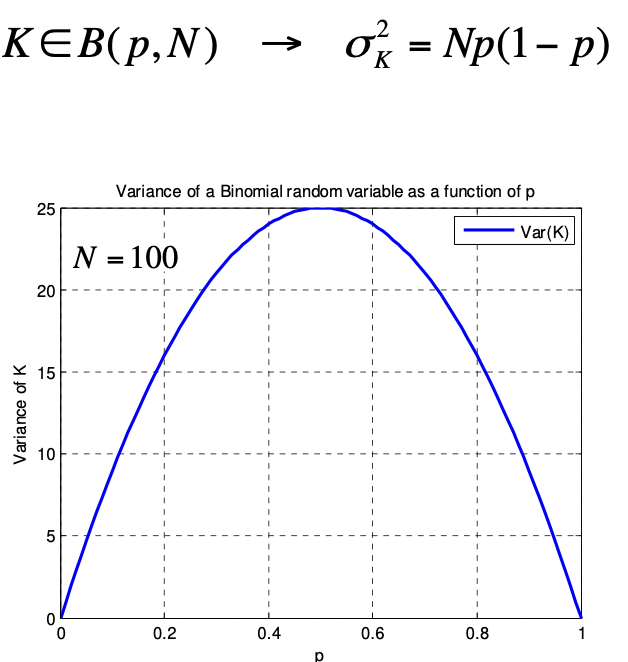
\includegraphics[width=0.5\linewidth]{Image/pdf 3/4.graph.png}
    \label{fig:placeholder}
\end{figure}
\item The variance of \(K\) is \(0\) when \(p=0\) or \(p=1\)(no spread of values around the mean, no uncertainty about the outcome of the trial). In this case, \(K\) assumes with probability 1 its mean value.
\item There is an important theorem about binomial random variables that we will use in the following: the \textbf{\underline{De Moivre-Laplace Theorem}}.
\item It is a special case of the \underline{\textbf{Central-Limit Theorem(CLT)}}: it states that the normal distribution may be used as an approximation to the binomial distribution under certain conditions.
\item In particular, the theorem shows that the \textbf{probability mass function(pmf)} of the random number \(K\) of "successes" observed in a series of \(N\) independent Bernoulli trials, each having probability \(p\) of success, converges to the \textbf{probability density function (pdf)} of the normal distribution with mean \(Np\) and variance \(Np(1-p)\):
\[
K \xrightarrow{N \rightarrow \infty} X, \quad \text{where} \quad X \in \mathcal{N}(Np, Np(1-p))
\]
\[
\text{convergence in distribution}
\]
\item Where \(Q\) is the \(Q\) error function.
\item In other words, if \(N\) is large enough, with good accuracy we can approximate the discrete r.v. \(K\) as a continuous Gaussian r.v. having the same mean and variance as \(K\):
\[
K \in \mathcal{B}(p, N), \quad \text{if } Np(1-p) \gg 1 : \quad K \in \mathcal{N}(Np, Np(1-p))
\]
\item The approximation requires \(Np(1-p)\gg 1\), but it is already good for \(Np(1-p)\geq10\).
\item \textbf{Standard Gaussian (or normal) r.v.}:
\[
X \in \mathcal{N}(0,1) \;\rightarrow\; f_X(x) = \frac{1}{\sqrt{2\pi}} \exp \left( -\frac{x^2}{2} \right)
\]

\[
\Phi(x) \triangleq F_X(x) = \Pr\{X \leq x\} = \int_{-\infty}^{x} f_X(z)\,dz = \frac{1}{\sqrt{2\pi}} \int_{-\infty}^{x} \exp \left( -\frac{z^2}{2} \right) dz
\]
\item \(\Phi(x)\) is not available in closed-form, it must be calculated numerically in MATLAB we use the script \textbf{normcdf.m}.
\item Frequently, we use the \textbf{Q functionc} defined as (in MATLAB: \textbf{qfunc.m}):
\[
Q(x) \triangleq \frac{1}{\sqrt{2\pi}} \int_{x}^{+\infty} \exp\left( -\frac{z^2}{2} \right) dz = 1 - \Phi(x)
\]
\item For a \textbf{Gaussin (or normal) r.v.} with given mean \(\eta\) and variance (\(\sigma^2\)):
\item For a \textbf{Gaussian (or normal) r.v.} having mean \(\eta\) and variance \(\sigma^2\):
\begin{figure}[H]
    \centering
    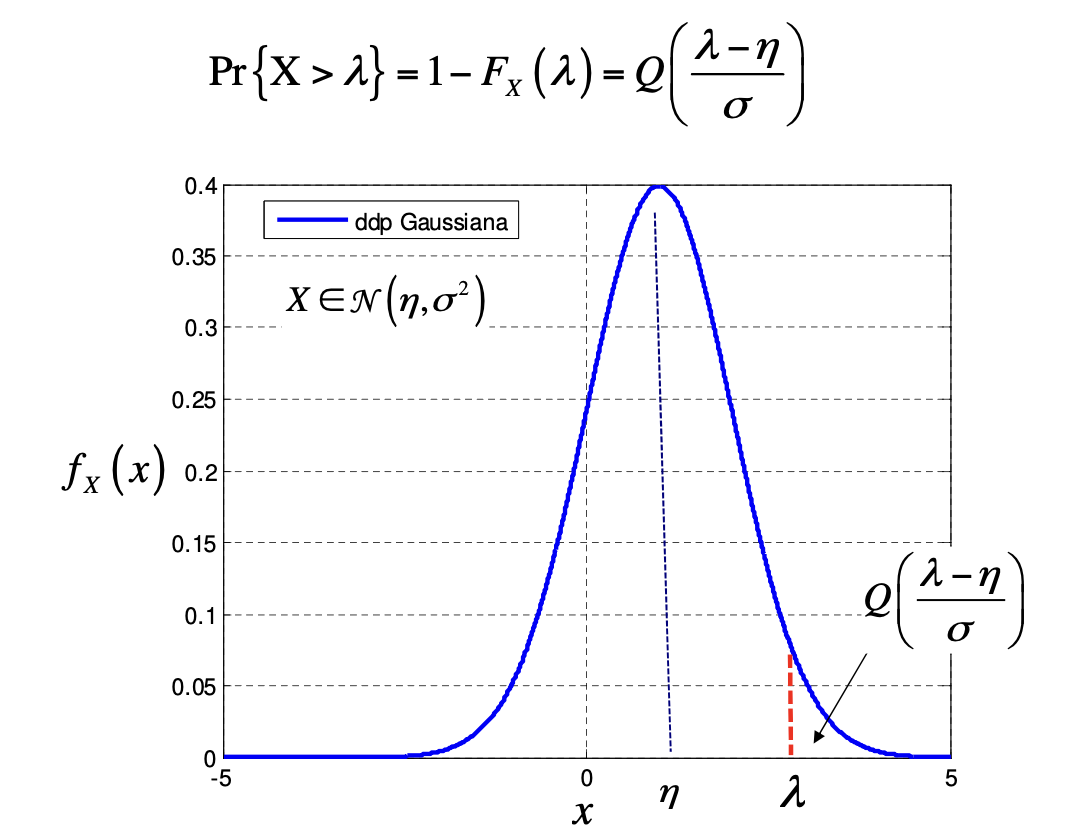
\includegraphics[width=0.55\linewidth]{Image/pdf 3/5. Gaussian.png}
    \label{fig:placeholder}
\end{figure}
\item In general, for a \textbf{Gaussian (or normal)} with mean \(\eta\) and variance \(\sigma^2\), the probability of any event we are interested can be easily calculated by using the \(Q\) function:
\[
\Pr\{a < X \leq b\}
= \int_{a}^{b} f_X(\alpha) d\alpha = F_X(b) - F_X(a)
\]

\[
= 1 - Q\left(\frac{b-\eta}{\sigma}\right) - \left[ 1 - Q\left(\frac{a-\eta}{\sigma}\right) \right]
\]

\[
= Q\left(\frac{a-\eta}{\sigma}\right) - Q\left(\frac{b-\eta}{\sigma}\right)
\]

\text{Note:} \quad Q(z) = 1 - Q(-z)
\item \textbf{Gaussian (or normal) r.v.} with mean \(\eta\) and variance \(\sigma^2\): the probability that the r.v. assumes a values that deviates from the mean value less than \(k\) times the standard deviation \(\sigma\) is given by:
\begin{figure}[H]
    \centering
    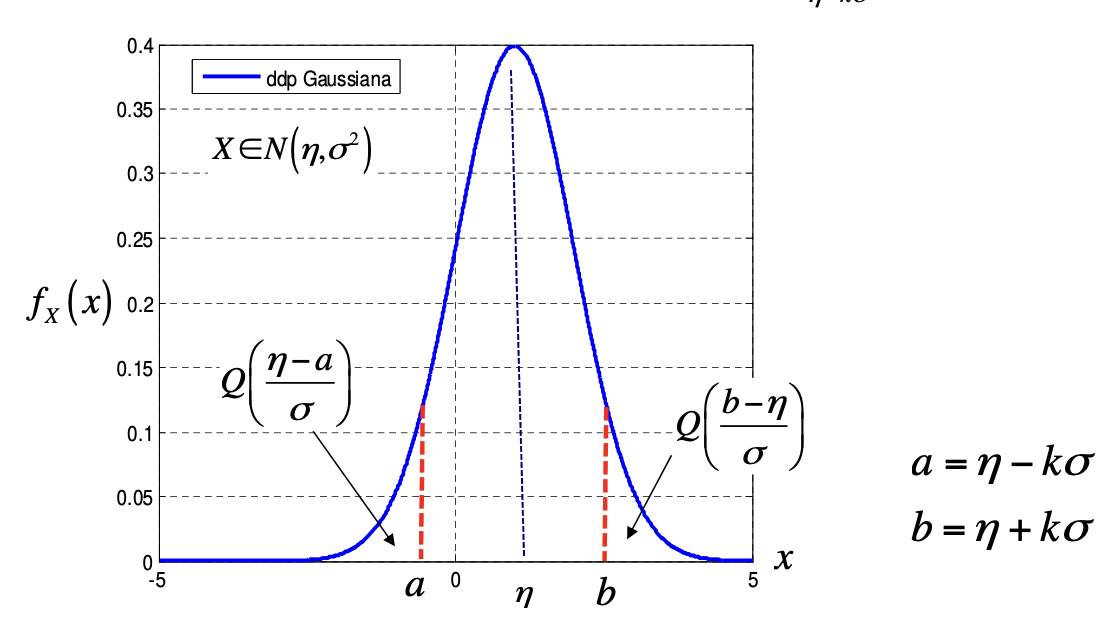
\includegraphics[width=0.75\linewidth]{Image/pdf 3/6.Gaussian 2 .png}
    \label{fig:placeholder}
\end{figure}
\item \textbf{Frequency of occurence F of an event A}:
\[
F \triangleq \frac{K}{N} = \frac{1}{N} \sum_{i=1}^{N} X_i
\qquad
\Bigl[ \text{Arithmetic mean of the observed data } \{ X_i \} \Bigr]
\]
\item \textbf{Mean value and variance of F}:
\[
\eta_F = E\{F\} = \frac{E\{K\}}{N} = p
\]

\[
\sigma_F^2 = E\left\{ (F - \eta_F)^2 \right\}
= E\left\{ \left( \frac{K}{N} - p \right)^2 \right\}
= E\left\{ \left( \frac{K - Np}{N} \right)^2 \right\}
\]

\[
= \frac{E\{(K-Np)^2\}}{N^2}
= \frac{\text{var}\{K\}}{N^2}
= \frac{p(1-p)}{N}
\]
\item \(F\) is a discrete r.v. that can assume values \(f_k=k/N\), for \(k=0,1,2,\cdots,N\):
\[
\text{Since} \quad p_F(f_k) \triangleq \Pr\left\{ F = f_k = \frac{k}{N} \right\} = \Pr\{ K = k \}
\implies
p_F(f_k) = p_K(k)\Big|_{k = N f_k}
\]
\item Hence, the \textbf{probability mass function(pmf)} of \(F\) is given by:
\[
p_K(k) = \Pr\{K = k\} = \binom{N}{k} p^k (1-p)^{N-k}, \quad 0 \leq k \leq N
\]
\[
p_F(f_k) = \Pr\{F = f_k\} 
= \binom{N}{Nf_k} p^{Nf_k} (1-p)^{N(1-f_k)}, \quad f_k = \frac{k}{N},\; 0 \leq k \leq N
\]
\begin{figure}[H]
    \centering
    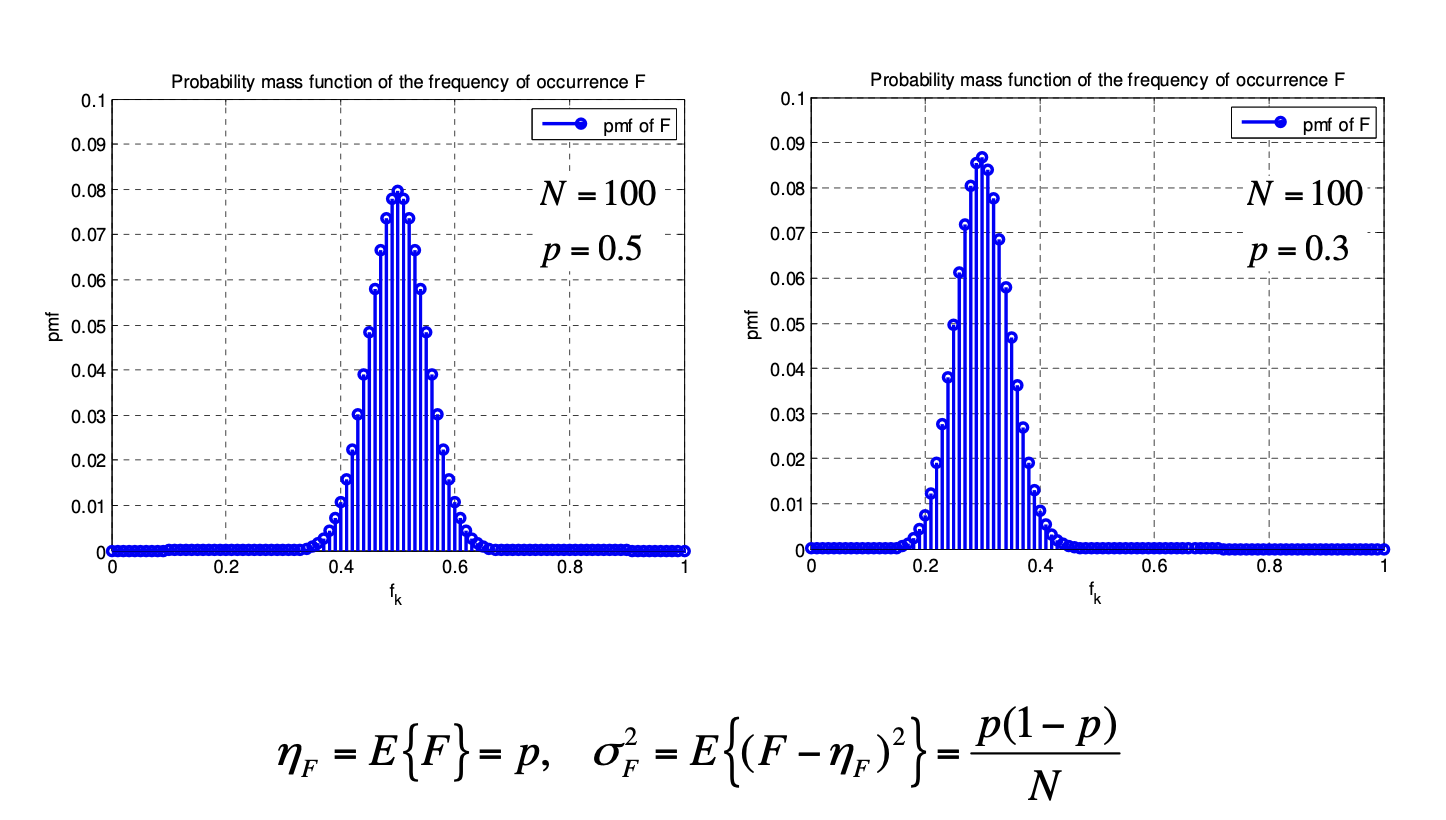
\includegraphics[width=0.6\linewidth]{Image/pdf 3/7.Ex_1.png}
    \label{fig:placeholder}
\end{figure}
\begin{figure}[H]
    \centering
    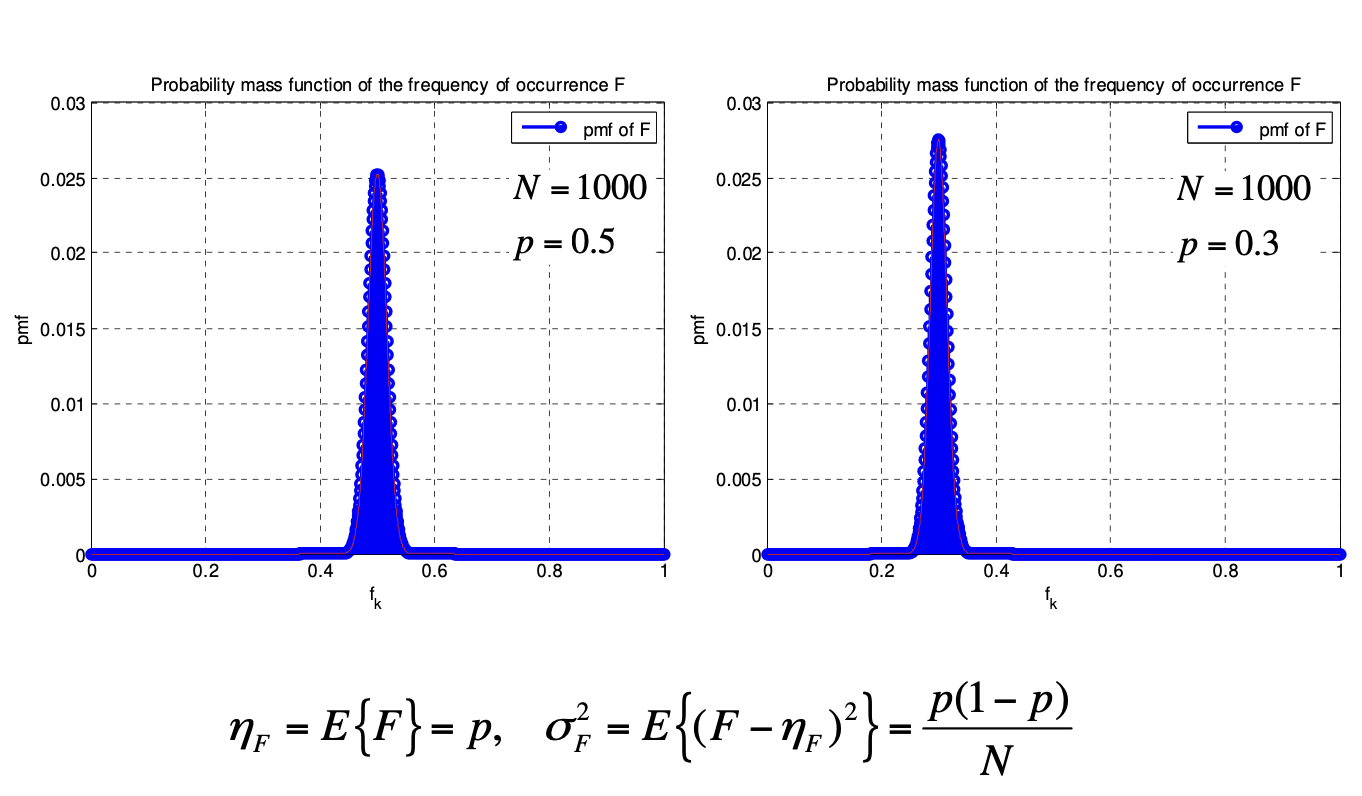
\includegraphics[width=0.6\linewidth]{Image/pdf 3/8.Ex_2.png}
    \label{fig:placeholder}
\end{figure}
\[
\eta_F=p,\quad \lim_{N\rightarrow\infty}\sigma^2_F=\lim_{N\rightarrow\infty}\frac{p(1-p)}{N}=0
\]
\item Hence: \[
F \xrightarrow{N \to \infty} p
\]
which means that the frequency of occurrence \(F\) of an event \(A\)(aritmetic mean of the \(N\) observed data \(X_i\)) converges to the probability \(p\) of the event (statistical mean of the \(X_i\)) when the numebr \(N\) of observed data grows to infinity.
\item The \textit{convergence} is both in mean square sense and in probability.
\item We have already seen that convergence in \textbf{mean square sense} implies convergence \textbf{in probability} thanks to the \textbf{Bienaymè-Tchebycheff inequality}:
\[
\text{\textbf{\underline{Bernoulli Theorem(or Large numbers law)}}}
\text{THe frequency of occurence \(F\) of an event \(A\), whose probability of occurrence is \(p\), converges in probability and in mean square sense to \(p\) when the number of N of independent trials goes to infinity}:
\]\[
\lim _{N\rightarrow\infty}F=p
\]
\item Hence, this suggest that {the probability \(p\)} can be estimated by calculating the frequency of occurence \(F\) of the event \(A\) over a number \(N\) of independent trials of the random experiment.
\item This estimator is \textbf{linear}, \textbf{unbiased} and \textbf{consistent}.
\item This estimator is \textbf{linear}, i.e. a linear function of the \(N\) data \{\(X_i\)\}, \textbf{unbiased} and \textbf{consistent}:
\[
\hat{p} = F = \frac{1}{N} \sum_{i=1}^N X_i
\]

\[
E\{\hat{p}\} = E\{F\} = \eta_F = p \qquad \rightarrow \text{unbiased}
\]

\[
MSE\{\hat{p}\} = E\left\{ (\hat{p} - p)^2 \right\} = E\left\{ (F - \eta_F)^2 \right\} = \sigma_F^2 = \frac{p(1-p)}{N}
\]

\[
\lim_{N\rightarrow\infty} MSE\{\hat{p}\}
= \lim_{N\rightarrow\infty} \sigma_F^2
= \lim_{N\rightarrow\infty} \frac{p(1-p)}{N}
= 0 
\qquad \rightarrow \text{consistent}
\]
\item \underline{De Moivre-Laplace theorem}\(\rightarrow\) the estimator is also \textbf{asymptotically Gaussian}:
\[
Np(1 - p) \gg 1 \;\; \Rightarrow \;\; \hat{p} \overset{a}{\in} \mathcal{N}\!\left(p, \frac{p(1 - p)}{N}\right)
\]
EXAMPLE: Series of graph in which, he shows the theorem.
\item \textit{Problem:} How to choose the number of observations \(N\)?
A possible criterion is to look for the minimum number of observed data which guarantees that the standard deviation of the error is a given fraction \(\alpha\) of the true value \(p\), e.g. \(\alpha=0.1\), i.e. \(10\%\) of \(p\). This is equivalent to say that the MSE should be lower than \(\alpha^2p^2\) :
\[
\sigma_\varepsilon = \sqrt{ E \left\{ (F - p)^2 \right\} } \leq \alpha p 
\rightarrow 
E\left\{ (F - p)^2 \right\} = MSE\left\{\hat{p}\right\} \leq \alpha^2 p^2
\]
\[
\rightarrow 
\frac{ E \left\{ (F - p)^2 \right\} }{ p^2 }
= E \left\{ \left( \frac{F - p}{p} \right)^2 \right\}
= E \left\{ \varepsilon_r^2 \right\} \leq \alpha^2
\]
\[
\text{Relative error:} \quad \varepsilon_r \triangleq \frac{F - p}{p} 
\implies
E\left\{ \varepsilon_r^2 \right\} = \frac{ E \left\{ (F - p)^2 \right\} }{ p^2 }
= \frac{ p(1-p) }{ Np^2 }
= \frac{1-p}{Np} \leq \alpha^2
\]
\item Example : \(\alpha =0.1\), i.e. the standard deviation of the error should be lower than \(10\%\) of \(p\).

\item \textbf{Rule of thumb}: \(N\) should be about two orders of magnitude greater than \(1/p\).
\item As a consequence, the lower is the probability \(p\) we want to estimate and the more data we need, if we want to achieve the require accuracy (\(10\%\) in this case).
\begin{figure}[H]
    \centering
    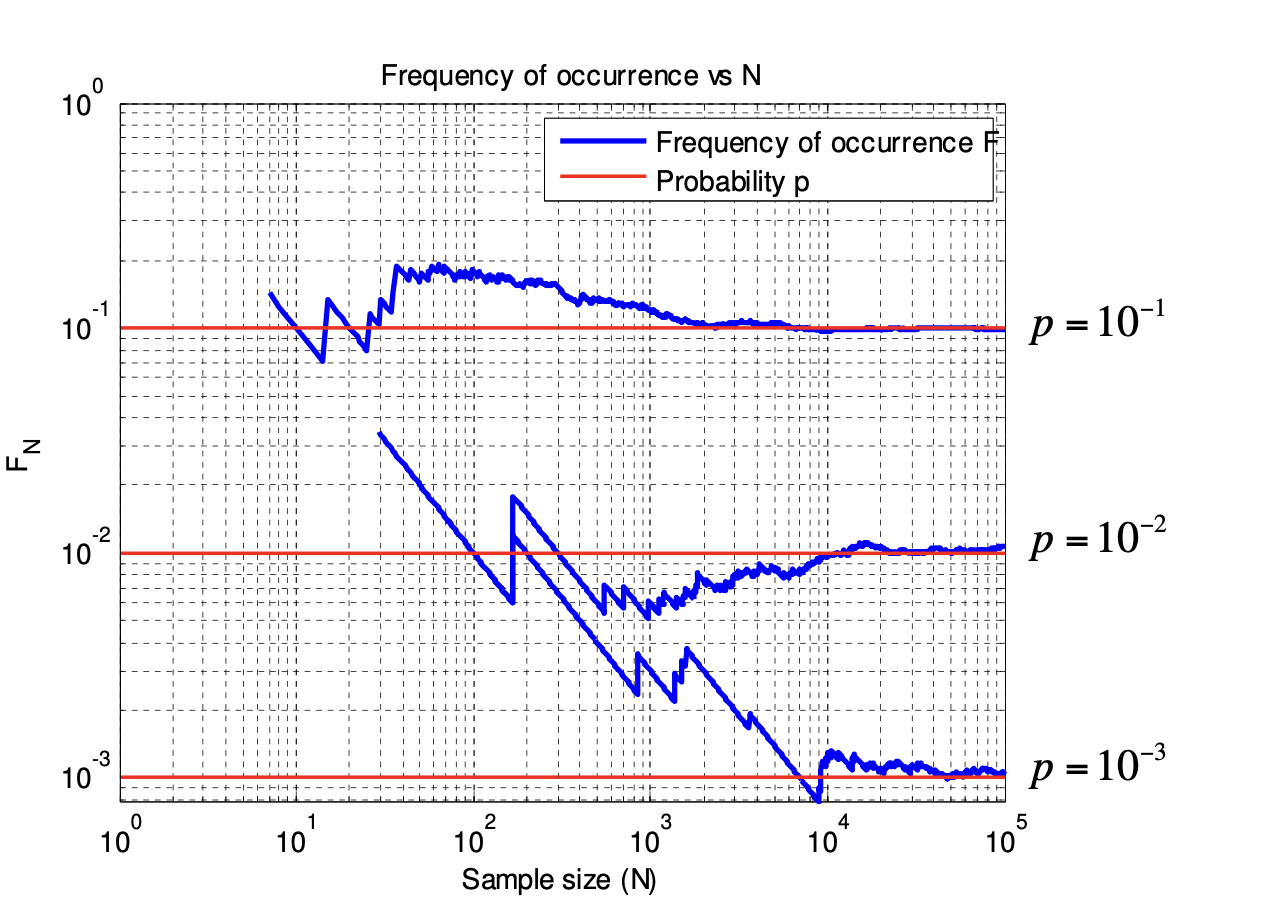
\includegraphics[width=0.55\linewidth]{Image/pdf 3/9.Ex_3.png}
    \label{fig:placeholder}
\end{figure}

\end{itemize}
\subsection{Measure of the Moments of a Random Variable}
\begin{itemize}
    \item We proved that if \(\{X_i\}'s\) are \(N\) independent and identically distributed (IID) binary random variables, when \(N\) goes to infinity the aritmetic mean converges to the statistical mean (ensamble mean):
    \[
F = \langle X_i \rangle = \frac{1}{N} \sum_{i=1}^{N} X_i 
\overset{N \to \infty}{\longrightarrow} 
E\left\{ X_i \right\} = p
\]
    \item The convergence is in mean square sense and in probability.
    \item \textbf{Question:} is it true only for IID binary random variables?
    \item As we will see in the following, the answer is NO. The only necessary condition is that the \(N\) r.v.'s are \textbf{identically distributed}.
    \item We can use this result to \textbf{estimate the mean value} of a general random variable \(X\)(not necessarily a binary r.v.).
    \item Let us define \(Z\) the aritmetic mean, also termed \textbf{Sample Mean}, of the \(\{X_i\}'s\), that are \(N\) realizations of the r.v. \(X\) of which we want to estimate the mean value \(\eta_X\).
    \item \(X\) can have \textbf{any probability density funcion(pdf)}, it should not necessarily be a binary r.v.; it can be either a discrete or a continuous r.v.
    \item We want to investigate if the \textbf{Sample Mean} of the \(N\) observed data can be used as an \textbf{estimator} of the \textbf{mean value} of \(X\).
    \[
\eta_X \triangleq E\left\{ \mathbf{X} \right\}, \qquad
\hat{\eta}_X = \langle X_i \rangle = \frac{1}{N} \sum_{i=1}^{N} X_i
\]
   \item To answer this question we have to calculate its \textbf{bias} and \textbf{MSE}.
   \item We assume that the \(N\) r.v. are \underline{identically distributed}, but not necessarily independent.
   \[
E\left\{\hat{\eta}_X\right\} = E\left\{ \frac{1}{N} \sum_{i=1}^{N} X_i \right\}
= \frac{1}{N} \sum_{i=1}^{N} E\left\{ X_i \right\}
= \frac{1}{N} \sum_{i=1}^{N} \eta_X = \eta_X
\]
   \item Hence, the mean value of the \textbf{Sample mean} is equal to the statistical mean of \(X\), as a consequence, the Sample Mean is an \textbf{unbiased} estimator of the mean of the r.v. \(X\).
   \item In other words, the mean value of hte estimation error is zero:
\[
\varepsilon \triangleq \eta_X - \hat{\eta}_X
\]
\[
E\left\{ \varepsilon \right\} = E\left\{ \eta_X - \hat{\eta}_X \right\}
= \eta_X - E\left\{ \hat{\eta}_X \right\} = \eta_X - \eta_X = 0
\]
\[
MSE\left\{ \hat{\eta}_X \right\} \triangleq E\left\{ \varepsilon^2 \right\}
= E\left\{ (\hat{\eta}_X - \eta_X )^2 \right\}
= \mathrm{var} \left\{ \hat{\eta}_X \right\}
\]
\[
MSE\left\{ \hat{\eta}_X \right\} = \mathrm{var}\left\{\hat{\eta}_X\right\}
= E\left\{ (\hat{\eta}_X - \eta_X)^2 \right\}
= E\left\{ \left( \frac{1}{N} \sum_{i=1}^{N} X_i - \eta_X \right)^2 \right\}
\]
\[
= E\left\{ \left( \frac{1}{N} \sum_{i=1}^{N} (X_i - \eta_X) \right)^2 \right\}
= \frac{1}{N^2} E \left\{ \left( \sum_{i=1}^N (X_i - \eta_X) \right)^2 \right\}
= \frac{1}{N^2} E \left\{ \sum_{i=1}^N (X_i - \eta_X) \sum_{k=1}^N (X_k - \eta_X) \right\}
\]
\[
= \frac{1}{N^2} \sum_{i=1}^N \sum_{k=1}^N E\left\{ (X_k - \eta_X)(X_i - \eta_X) \right\}
= \frac{1}{N^2} \sum_{i=1}^N \sum_{k=1}^N c_{X_k X_i}
\]
\[
= \frac{1}{N^2} \sum_{i=1}^N \sigma_X^2 + \frac{1}{N^2} \sum_{i=1}^N \sum_{k=1,\,k\neq i}^N c_{X_k X_i}
= \frac{\sigma_X^2}{N} + \frac{1}{N^2} \sum_{i=1}^N \sum_{k=1,\,k\neq i}^N c_{X_k X_i}
\]
\[
\text{where} \quad c_{X_k X_i} \triangleq \mathrm{cov}\left\{ X_k, X_i \right\}
= E\left\{ (X_k - \eta_X)(X_i - \eta_X) \right\}
\]
\item If the \(\{X_i\}'s\) are \underline{independent}, they are also \underline{uncorrelated}, so we have :
\[
c_{X_k X_i} = \mathrm{cov}\left\{ X_k, X_i \right\}
= E\left\{ (X_k - \eta_X)(X_i - \eta_X) \right\}
= \begin{cases}
\sigma_X^2 & i = k \\
0 & i \neq k
\end{cases}
\]
\[
MSE\left\{ \hat{\eta}_X \right\} = \frac{\sigma_X^2}{N}
\]
\item If the variance of \(X\) is finite, the MSE of the Sample Mean tends to zero when \(N\) goes to infinity!

\[
E\left\{\hat{\eta}_X\right\} = \eta_X  \longrightarrow \text{unbiased}
\]
\[
MSE\left\{ \hat{\eta}_X \right\}
= E\left\{ (\hat{\eta}_X - \eta_X)^2 \right\}
= \frac{\sigma_X^2}{N}
\]
\[
\lim_{N \to \infty} MSE\left\{ \hat{\eta}_X \right\}
= \lim_{N \to \infty} \frac{\sigma_X^2}{N} = 0
 \longrightarrow \text{consistent}
\]
\item In summary, we proved that \underline{if the variance of X is finite} and the observed data are IID, the \textbf{Sample Mean} converges in mean square sense, and so also in probability, to the statistical mean of X. We will analyze separately the case of \underline{dependent} data.
\item The \textbf{mean square value} of the \textbf{\underline{relative error}} is :
\[
\left\{
\begin{aligned}
    &\varepsilon_r \triangleq \frac{\varepsilon}{\eta_X} = \frac{\eta_X - \hat{\eta}_X}{\eta_X} \\[2ex]
    &\sigma^2_{\varepsilon_r} = E \left\{ \left( \frac{\eta_X - \hat{\eta}_X}{\eta_X} \right)^2 \right\}
    = \frac{E \left\{ (\eta_X - \hat{\eta}_X)^2 \right\} }{\eta_X^2}
    = \frac{MSE\left\{\hat{\eta}_X\right\}}{\eta_X^2}
    = \frac{\sigma_X^2}{\eta_X^2 N}
    = \frac{1}{\gamma N}
\end{aligned}
\right.
\]
\[
\text{where} \quad \gamma \triangleq \frac{\eta_X^2}{\sigma_X^2} \quad\text{is a sort of SNR}
\]
\begin{figure}[H]
    \centering
    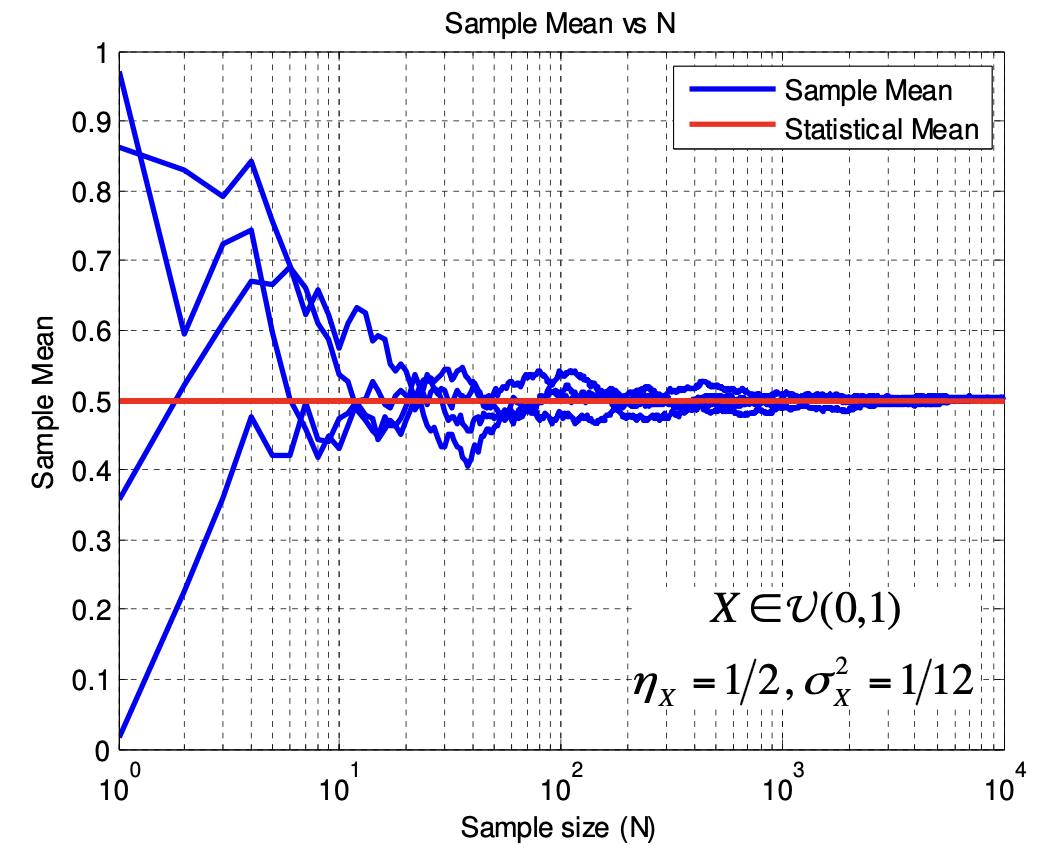
\includegraphics[width=0.55\linewidth]{Image/pdf 3/10.Stat_VS_Sample.png}
    \label{fig:placeholder}
\end{figure}
   \item If \(X\) is a Gaussian r.v., since the \textbf{Sample Mean} \(Z\) is a linear combination of Gaussian r.v.'s, it is also Gaussian distributed:
   \[
\mathbf{X} \in \mathcal{N} \left(\eta_X, \sigma_X^2 \right)
\implies
Z = \frac{1}{N} \sum_{i=1}^N X_i\quad \text{is a Gaussian r.v.}
\]
\[
Z \in \mathcal{N} \left(\eta_X, \frac{\sigma_X^2}{N} \right)
\]
\item Even if \(X\) is not Gaussian distributed, thanks to \textbf{\underline{Central-limit Theorem}}, for large \(N\) can be approximate \(Z\) as a Gaussian random variable.
\item Even if \(X\) is not Gaussian distributed, thanks to the \textbf{\underline{Central-limit theorem}}, \(Z\) is asymptotically distributed, i.e. for \(N\rightarrow\infty\).
\item Hence, if \(N\) is large, even if finite, the approximation is accurate and we can rely on the gaussian assumption to calculate the probabilities of events of interest:
\[
\hat{\eta}_X = Z = \frac{1}{N} \sum_{i=1}^{N} X_i
\overset{a}{\in} \mathcal{N} \left( \eta_X, \frac{\sigma_X^2}{N} \right)
\]

\[
\Pr \left\{ \left| \hat{\eta}_X - \eta_X \right| \leq k \frac{\sigma_X}{\sqrt{N}} \right\}
= 1 - 2 Q(k) \approx
\begin{cases}
0.683 & k=1 \\
0.956 & k=2 \\
0.997 & k=3 \\
\end{cases}
\]
The length of \(k\frac{\sigma_X}{\sqrt{N}}\) goes to \(0\) when \(N\) goes to infinity.
\begin{figure}[H]
    \centering
    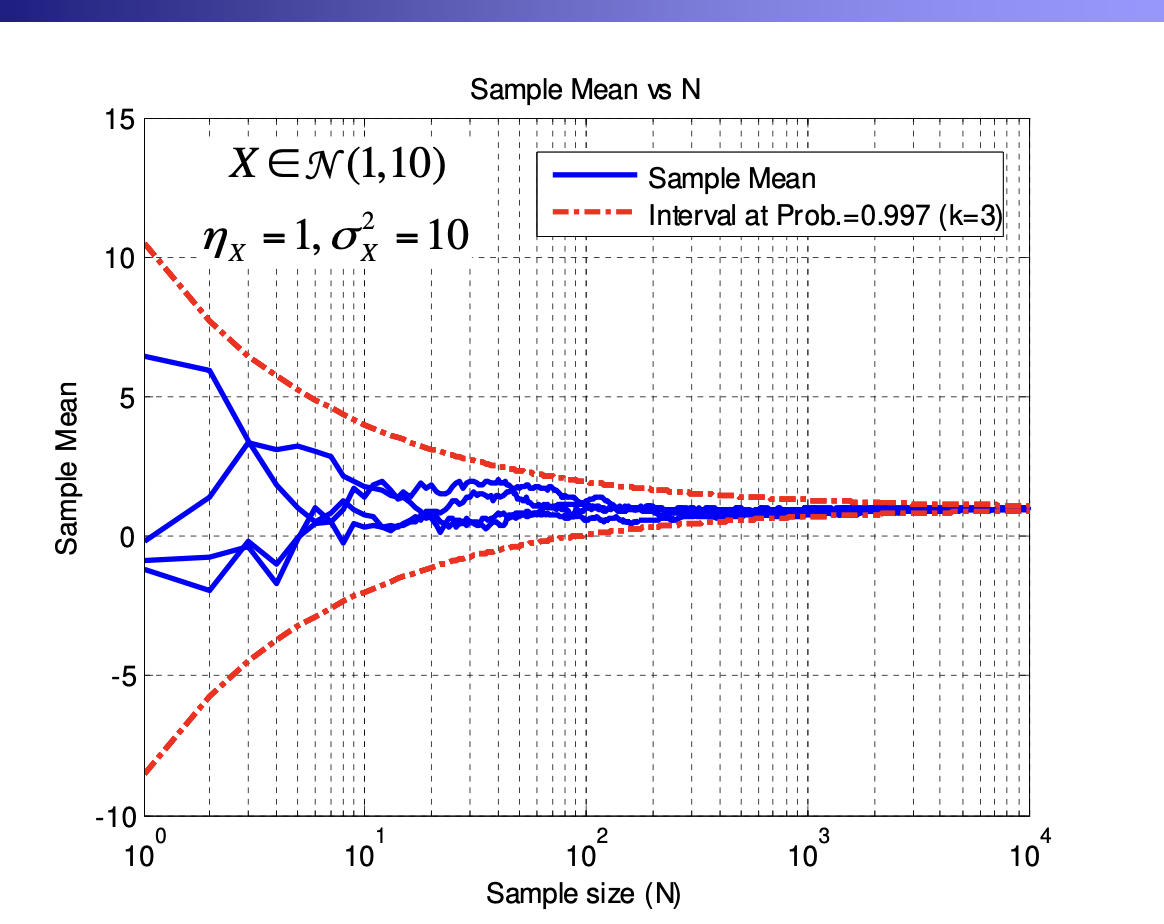
\includegraphics[width=0.55\linewidth]{Image/pdf 3/11.Ex_for_K=3.png}
    \label{fig:placeholder}
\end{figure}
\item How to choose \(N\)? One possible criterion is to choose the minimum value which guarantees that \underline{the standard deviation of the relative error} is lower than a certain value, e.g. \(10\%\):
\[
\sigma_{\varepsilon_r} = \sqrt{ E \left\{ \left( \frac{\eta_X - \hat{\eta}_X}{\eta_X} \right)^2 \right\} }
= \sqrt{ \frac{1}{N \gamma} } \leq 0.1
\implies N \geq \frac{100}{\gamma}
\]
\item The value of \(N\) is inversely proportional to the ratio \(\gamma\), which is a sort of SNR:
\[
\gamma\triangleq\frac{\eta_X^2}{\sigma_X^2}
\]
\item If we know the pdf og \(Z\), we can calculate the minimum value of \(N\) such that the absolute value of the relative error is lower of a given value \(\delta\), e.g. \(\delta=0.1\) i.e., with a desired probability \(\alpha\).
\[
\hat{\eta}_X \overset{a}{\in} \mathcal{N} \left(\eta_X, \frac{\sigma_X^2}{N}\right)
\]

\[
\Pr\left\{ \left| \frac{\hat{\eta}_X - \eta_X}{\eta_X} \right| \leq \delta \right\}
= \Pr\left\{ \left| \hat{\eta}_X - \eta_X \right| \leq \delta \eta_X \right\} = \alpha
\]

\[
\Pr\left\{ \left| \hat{\eta}_X - \eta_X \right| \leq \delta \eta_X \right\}
= 1 - 2Q\left( \frac{\delta \eta_X \sqrt{N}}{\sigma_X} \right) = \alpha
\]

\[
\implies \frac{\delta \eta_X \sqrt{N}}{\sigma_X}
= Q^{-1} \left( \frac{1-\alpha}{2} \right)
\implies N = \left[ \frac{\sigma_X}{\delta \eta_X} Q^{-1}\left( \frac{1-\alpha}{2} \right) \right]^2
\]
If we try to set \(\delta=0.1\) and \(\alpha=0.95\):
\[
N = \left[ \frac{\sigma_X}{0.1\, \eta_X} Q^{-1}\left( \frac{1-0.95}{2} \right) \right]^2
= \frac{10^2 \sigma_X^2}{\eta_X^2} [1.96]^2
= 384 \cdot \frac{\sigma_X^2}{\eta_X^2}
= \frac{384}{\gamma}
\]
The value of \(N\) is again inversely proportional to the ratio \(\gamma\). Clearly, if this ratio does not return an integer number, we choose the smallest integer grater than this ratio.\\
Clearly, if this ratio does not return an integer number, we choose the smallest integer greater than this ratio.

\item Let us now investigate the behavior of the \textbf{Sample Mean} in the case of \textbf{depedent data}, i.e. the \(N\) observed samples are identically distributed but \textbf{not} independent:

\[
\hat{\eta}_X = \frac{1}{N} \sum_{i=1}^N X_i \qquad
E\left\{\hat{\eta}_X\right\} =
E\left\{\frac{1}{N} \sum_{i=1}^N X_i\right\} =
\frac{1}{N} \sum_{i=1}^N E\left\{X_i\right\} =
\eta_X
\]
\item Hence, independently from the fact that \(\{X_i\}\) are independent or not, the \textbf{Sample mean} is an \textbf{unbiased estimator} of the statistical mean of X.

\item Let us now calculate the MSE : since the estimator is unbiased, the MSE coincides with the variance of the estimator.

\item We already derived the following result for the MSE:
\[
MSE\left\{ \hat{\eta}_X \right\}
= \frac{1}{N^2} \sum_{i=1}^{N} \sum_{j=1}^{N} c_{X_i X_j}
= \frac{\sigma_X^2}{N}
+ \frac{1}{N^2} \sum_{i=1}^{N} \sum_{\substack{j=1 \\ j \neq i}}^{N} c_{X_j X_i}
\]

\[
c_{X_i X_j} \triangleq E\left\{ (X_i - \eta_X)(X_j - \eta_X) \right\},\quad i, j = 1,2, \cdots, N
\]
\item The \textbf{Sample Mean} is a \textbf{consistent} estimator if and ony if (iff):
\[
\lim_{N \to \infty} MSE\left\{\hat{\eta}_X\right\}
= \lim_{N \to \infty} \frac{1}{N^2} \sum_{i=1}^{N} \sum_{j=1}^{N} c_{X_i X_j}
= \lim_{N \to \infty} \left( \frac{\sigma_X^2}{N}
+ \frac{1}{N^2} \sum_{i=1}^{N} \sum_{\substack{j=1 \\ j \neq i}}^{N} c_{X_j X_i} \right)
= 0
\]
\item When does this happen? \textbf{The independence assumption is not necessary}

\item We proved that if the \(\{X_i\}\) are IID we have that :
\[
\left\langle X_i \right\rangle = \frac{1}{N} \sum_{i=1}^N X_i \xrightarrow{N \to \infty} E\left\{ X_i \right\}, \quad \text{if} \quad \mathrm{var}\left\{X_i\right\} < +\infty
\]
\item How can we extend this result if we want to estimate other \textbf{statistical indexes}, e.g. the \textit{variance}, the \textit{skewness} or the \textit{kurtosis}?
\item If we define a new r.v. \(S=g(X)\) and we apply the previous results to \(S\) we get:
\[
\left\langle S_i \right\rangle = \frac{1}{N} \sum_{i=1}^N S_i \xrightarrow{N \to \infty} E\left\{ S_i \right\}, \quad \text{if} \quad \mathrm{var}\left\{ S_i \right\} < +\infty
\]

\[
\left\langle g(X_i) \right\rangle = \frac{1}{N} \sum_{i=1}^N g(X_i) \xrightarrow{N \to \infty} E\left\{ g(X_i) \right\}, \quad \text{if} \quad \mathrm{var}\left\{ g(X_i) \right\} < +\infty
\]
In the case we want to estimate the \textbf{variance} :
\[
\sigma_X^2 = E\left\{(X - \eta_X)^2\right\}
\implies
S \triangleq g(X) = (X - \eta_X)^2
\]
\item The previous result suggests to estimate the variance as follows:
\[
\hat{\sigma}_X^2 = \left\langle (X_i - \eta_X)^2 \right\rangle = \frac{1}{N} \sum_{i=1}^N (X_i - \eta_X)^2
\]
\item The problem is that also the mean is usually unknown, so we should replace the mean with its estimate, i.e. the Sample Mean:
\[
\hat{\sigma}_X^2 = \left\langle (X_i - \hat{\eta}_X)^2 \right\rangle
= \frac{1}{N} \sum_{i=1}^N (X_i - \hat{\eta}_X)^2
\]
\[
\text{where} \qquad \hat{\eta}_X = \frac{1}{N} \sum_{k=1}^{N} X_k
\]

\item The estimator of the variance we derived is called \underline{\textbf{Sample Variance}}.
\item To derive the bias, it is useful to express it in a different way:
\[
\begin{aligned}
\hat{\sigma}_X^2 &= \frac{1}{N} \sum_{i=1}^N (X_i - \hat{\eta}_X)^2 \\
&= \frac{1}{N} \sum_{i=1}^N X_i^2 - 2 \cdot \frac{1}{N} \sum_{i=1}^N X_i \hat{\eta}_X + \frac{1}{N} \sum_{i=1}^N \hat{\eta}_X^2 \\
&= \frac{1}{N} \sum_{i=1}^N X_i^2 - 2 \hat{\eta}_X \cdot \frac{1}{N} \sum_{i=1}^N X_i + \hat{\eta}_X^2 \\
&= \frac{1}{N} \sum_{i=1}^N X_i^2 - \hat{\eta}_X^2
\end{aligned}
\]

\item We derive nw the mean calue and the variance of the \textbf{Sample Variance}, and then its bias MSE.\\
\textbf{Assumption}: the observed data \(\{X_i\}\) are IID.
\item \textbf{Mean value and variance of the Sample Variance}:
\[
\begin{aligned}
\hat{\sigma}_X^2 &= \frac{1}{N} \sum_{i=1}^{N} X_i^2 - \hat{\eta}_X^2 \\[1.5ex]
E \left\{ \hat{\sigma}_X^2 \right\} &= E \left\{ \frac{1}{N} \sum_{i=1}^N X_i^2 - \hat{\eta}_X^2 \right\}
= E \left\{ \frac{1}{N} \sum_{i=1}^N X_i^2 \right\} - E \left\{ \hat{\eta}_X^2 \right\} \\[1.5ex]
&= \frac{1}{N} \sum_{i=1}^N E \left\{ X_i^2 \right\}
- \left( \operatorname{var}\left\{ \hat{\eta}_X \right\} + \left( E \left\{ \hat{\eta}_X \right\} \right)^2 \right) \\[1.5ex]
&= \frac{1}{N} \sum_{i=1}^N \left( \sigma_X^2 + \eta_X^2 \right)
- \left( \frac{\sigma_X^2}{N} + \eta_X^2 \right) \\[1.5ex]
&= \sigma_X^2 - \frac{\sigma_X^2}{N}
= \left(1-\frac{1}{N}\right) \sigma_X^2
\end{aligned}
\]

\item The \textbf{Sample Variance} is a \textbf{biased} estimator of the variance:
\[
E \left\{ \hat{\sigma}_X^2 \right\} = \sigma_X^2 \left( 1 - \frac{1}{N} \right) \neq \sigma_X^2
\]

\[
b \left\{ \hat{\sigma}_X^2 \right\} \triangleq E \left\{ \varepsilon \right\}
= E \left\{ \sigma_X^2 - \hat{\sigma}_X^2 \right\}
= \sigma_X^2 - \sigma_X^2 \left( 1 - \frac{1}{N} \right)
= \frac{\sigma_X^2}{N} \neq 0
\]

\item The \textbf{Sample variance} is \textbf{biased} but \textbf{asymptotically unbiased}:
\[
\lim_{N\rightarrow+\infty}b\{\hat{\sigma_X^2}\}=\lim_{N\rightarrow+\infty}\frac{\sigma_X^2}{N}=0
\]

\item The derivation of the \textbf{variance} of the \textbf{Sample Variance} is quite tedious, but not conceptually difficult. We skip the derivation and we provide the result:

\[
\begin{aligned}
\hat{\sigma}_X^2 &= \frac{1}{N} \sum_{i=1}^N (X_i - \hat{\eta}_X)^2 \\[1.5ex]
E\left\{\hat{\sigma}_X^2\right\} &= \sigma_X^2 \left(1 - \frac{1}{N}\right) \\[1.5ex]
\operatorname{var}\left\{\hat{\sigma}_X^2\right\} &= E\left\{\left(\hat{\sigma}_X^2 - E\left\{\hat{\sigma}_X^2\right\}\right)^2\right\}
= E\left\{\left(\frac{1}{N} \sum_{i=1}^N (X_i - \hat{\eta}_X)^2 - \sigma_X^2 \left(1 - \frac{1}{N}\right)\right)^2\right\} \\[1.5ex]
&= \frac{\mu_X(4) - \sigma_X^4}{N}
- \frac{2 \left(\mu_X(4) - 2\sigma_X^4\right)}{N^2}
+ \frac{\mu_X(4) - 3\sigma_X^4}{N^3}
\end{aligned}
\]
\[
\mu_X(4) \triangleq E\left\{(X - \eta_X)^4\right\} \text{ is the 4th order central moment of X}
\]
\item if the 4th order central moment is finite, i.e. \(\mu_X(4)<+\infty\)
\[
\lim_{N \to \infty} \operatorname{var} \left\{ \hat{\sigma}_X^2 \right\}
= \lim_{N \to \infty} \left[
\frac{\mu_X(4) - \sigma_X^4}{N}
- \frac{2\left(\mu_X(4) - 2\sigma_X^4\right)}{N^2}
+ \frac{\mu_X(4) - 3\sigma_X^4}{N^3}
\right] = 0
\]

\[
b\left\{\hat{\sigma}_X^2\right\} = \frac{\sigma_X^2}{N}
\]

\[
MSE\left\{\hat{\sigma}_X^2\right\}
= \operatorname{var}\left\{\hat{\sigma}_X^2\right\}
+ \left(b\left\{\hat{\sigma}_X^2\right\}\right)^2
\xrightarrow{N \to \infty} 0
\]
\item In summary, under the IID assumption, the \textbf{Sample Variance} is a \underline{\textbf{consistent}} estimator of the variance.\\
It is \textbf{biased} but \textbf{asymptotically unbiased}.

\item \underline{If \(X\) is a \textbf{Gaussian} random variable}:
\[
\begin{aligned}
& X \in \mathcal{N}(\eta_X, \sigma_X^2) \qquad \rightarrow \qquad \mu_X(4) = 3\sigma_X^4 \\[2ex]
&\operatorname{var}\left\{ \hat{\sigma}_X^2 \right\}
= \frac{2\sigma_X^4}{N} - \frac{2\sigma_X^4}{N^2}
= \frac{2\sigma_X^4}{N} \left( 1 - \frac{1}{N} \right)
\mathrel{\overset{N \gg 1}{\approx}} \frac{2\sigma_X^4}{N} \\[2ex]
& b\left\{\hat{\sigma}_X^2\right\} = \frac{\sigma_X^2}{N} \\[2ex]
& MSE\left\{\hat{\sigma}_X^2\right\}
= \operatorname{var}\left\{\hat{\sigma}_X^2\right\} + \left( b\left\{\hat{\sigma}_X^2\right\} \right)^2
= \frac{2\sigma_X^4}{N} \left( 1 - \frac{1}{N} \right) + \frac{\sigma_X^4}{N^2} \\[1.5ex]
& \hspace{5em} = \frac{2\sigma_X^4}{N} \left( 1 - \frac{1}{2N} \right)
\mathrel{\overset{N \gg 1}{\approx}} \frac{2\sigma_X^4}{N}
\end{aligned}
\]
\item How can we get an \textbf{unbiased} estimator of the variance?

\[
\tilde{\sigma}_X^2 = \alpha \hat{\sigma}_X^2 = \frac{\alpha}{N} \sum_{i=1}^N (X_i - \hat{\eta}_X)^2, \qquad \text{where } \alpha \text{ is such that } E\left\{ \tilde{\sigma}_X^2 \right\} = \sigma_X^2 
\]
\[
E\left\{ \tilde{\sigma}_X^2 \right\} = E\left\{ \alpha \hat{\sigma}_X^2 \right\} = \alpha \sigma_X^2 \left( 1 - \frac{1}{N} \right) = \sigma_X^2 \qquad \Rightarrow \qquad \alpha = \left(1 - \frac{1}{N}\right)^{-1} = \frac{N}{N-1}
\]
\[
\tilde{\sigma}_X^2 = \frac{N}{N-1} \hat{\sigma}_X^2 = \frac{1}{N-1} \sum_{i=1}^N (X_i - \hat{\eta}_X)^2 \qquad \text{[unbiased estimator of } \sigma_X^2\text{]}
\]

\item We observe that if \(N\gg1\) there is no significant difference between the two estimators(biased and unbiased). The difference may be significant for small \(N\).
\[
\begin{aligned}
\tilde{\sigma}_X^2 &= \frac{1}{N-1} \sum_{i=1}^N (X_i - \hat{\eta}_X)^2 = \frac{N}{N-1} \hat{\sigma}_X^2 \\[1ex]
MSE\left\{ \tilde{\sigma}_X^2 \right\} &= \operatorname{var}\left\{\tilde{\sigma}_X^2\right\} + \left( b\left\{ \tilde{\sigma}_X^2 \right\} \right)^2 \\[1ex]
&= \operatorname{var} \left\{ \frac{N}{N-1} \hat{\sigma}_X^2 \right\} \\
&= \left( \frac{N}{N-1} \right)^2 \operatorname{var} \left\{ \hat{\sigma}_X^2 \right\} \\[1ex]
&= \left( \frac{N}{N-1} \right)^2 \frac{2\sigma_X^4}{N} \left( 1 - \frac{1}{N} \right) \\[1ex]
&= \frac{2\sigma_X^4}{N-1} \\[1ex]
MSE\left\{ \tilde{\sigma}_X^2 \right\} 
&= \frac{2\sigma_X^4}{N-1} = \frac{2\sigma_X^4}{N} \left( 1 + \frac{1}{N-1} \right) > \frac{2\sigma_X^4}{N} \left( 1 - \frac{1}{2N} \right) = MSE\left\{ \hat{\sigma}_X^2 \right\}
\end{aligned}
\]

\noindent The unbiased estimator has higher MSE than the biased one, hence its less efficient.

\item In \underline{summary}, we proved that
\[
\left\langle g(X_i) \right\rangle = \frac{1}{N} \sum_{i=1}^{N} g(X_i)
\xrightarrow{N \to \infty}
E\left\{ g(X_i) \right\}
\quad \text{if} \quad \mathrm{var}\left\{ g(X_i) \right\} < +\infty
\]

\item This suggest that if we want to estimate a parameter \(\delta=E\{g(X)\}\), and we can observe \(N\) independent realizations of the r.v. \(X\), a \underline{consistent} estimator of \(\delta\) is given by the \textbf{Sample Estimator}:
\[
\hat{\delta} = \left\langle g(X_i) \right\rangle = \frac{1}{N} \sum_{i=1}^{N} g(X_i)
\xrightarrow{N \to \infty}
\delta = E\left\{ g(X_i) \right\}
\quad \text{if} \quad \mathrm{var} \left\{ g(X_i) \right\} < +\infty
\]
\item The assumption that the \(N\) data \(\{X_i\}\) are independent is a sufficient condition for consistency, but not necessary.

\item We can use Sample Estimators to estimate any ordinary/central moment of X.
\[
\delta = E\left\{ g(X_i) \right\}, \quad \mathrm{var}\left\{ g(X_i) \right\} < +\infty, \qquad \hat{\delta} = \frac{1}{N} \sum_{i=1}^{N} g(X_i)
\]
\[
E \left\{ \hat{\delta} \right\}
= E \left\{ \frac{1}{N} \sum_{i=1}^{N} g(X_i) \right\}
= \frac{1}{N} \sum_{i=1}^{N} E \left\{ g(X_i) \right\}
= \frac{1}{N} \sum_{i=1}^{N} \delta = \delta 
\]
\[
\mathrm{var}\left\{ \hat{\delta} \right\}
= \mathrm{var}\left\{ \frac{1}{N} \sum_{i=1}^{N} g(X_i) \right\}
= \frac{1}{N^2} \sum_{i=1}^{N} \mathrm{var}\left\{ g(X_i) \right\}
= \frac{\mathrm{var}\left\{ g(X_i) \right\}}{N} 
\]
\[
\lim_{N \to \infty} MSE\left\{ \hat{\delta} \right\}
= \lim_{N \to \infty} \mathrm{var}\left\{ \hat{\delta} \right\}
= \lim_{N \to \infty} \frac{\mathrm{var}\left\{ g(X_i) \right\}}{N} = 0
\]
\item Where we used the fact that the \(N\) observed data \(\{X_i\}\) are independent and identically distributed (IID).

\item \textbf{Ordinary moments}: 
\[
m_X(n) \triangleq E\left\{ X^n \right\}
\implies
\hat{m}_X(n) = \frac{1}{N} \sum_{i=1}^{N} X_i^n
\]
\item \textbf{Central moments}:
\[
\mu_X(n) \triangleq E \left\{ (X - \eta_X)^n \right\}
\implies
\hat{\mu}_X(n) = \frac{1}{N} \sum_{i=1}^{N} (X_i - \hat{\eta}_X)^n
\]
\noindent \(\hat{\eta}_X\) introduces a bias.

\item It is important to note that in the Gaussian case (but it is true in general):
\[
\frac{2\sigma_X^4}{N} \left(1 - \frac{1}{2N}\right) > \frac{\sigma_X^2}{N}
\;\;\; \rightarrow \;\;\;
MSE\left(\hat{\sigma}_X^2\right) > MSE\left(\hat{\eta}_X\right)
\]
\item Given the data size \(N\), the MSE is larger for higher-order moments. In other word, \underline{the higher is the }\\
\noindent \underline{order \(n\) of the moment we want to estimate and the more data we need to achieve a desired} \\ 
\noindent \underline{estimation accuracy}.
\newpage
\[
\textbf{Definition of Skewness and Kurtosis}
\]
\vspace{0.5em}
\[
\gamma_{3X} \triangleq \frac{\mu_X(3)}{\left( \mu_X(2) \right)^{3/2}} \hspace*{3em} \gamma_{4X} \triangleq \frac{\mu_X(4)}{\left( \mu_X(2) \right)^{2}} - 3
\]
\vspace{0.5em}
\[
\text{where } \mu_X(2)=\sigma_X^2\text{ is a variance of X}
\]

\item The \textit{Skewness} is the \underline{normalized} 3rd order central moment of a r.v., it is a measure of asymmetry of a distribution.
\item All simmetric distributions have zero \textit{skewness}, so the \textit{skewness} of a Gaussian r.v. is zero.
\item If the \textit{skewness} is different from zero (neglecting the measurement errors), the observed data cannot be Gaussian. 
\[
X \in \mathcal{N}(\eta_X, \sigma_X^2) 
\rightarrow 
\mu_X(4) = 3\sigma_X^4
\rightarrow 
\frac{\mu_X(4)}{\left(\mu_X(2)\right)^2} = 3
\rightarrow 
\gamma_{4X} = 0
\]
\item The \textit{kurtosis} is the \underline{normalized} 4th order central moment of a r.v. scaled in such a way that is zero for a Gaussian r.v.
\item It is a measure of \textit{flatness} of the distribution w.r.t the Gaussian one.
\item If the \textit{kurtosis} is positive the pdf has longer tails than the Gaussian one, so the probability to observe large values is higher than in the Gaussian case.\\
These kind of pdf's are called \textbf{heavy-tailed distributions}(e.g. the Laplace, the Weibull, the log-normal, the K, the t-distribution re heavy-tailed).
\item The \textit{skewness} and \textit{kurtosis} are indicators of non Gaussianity of the data: if they are different from zero the data cannot be Gaussian distributed.
\item We can build statistical test based on the sample estimated of the \textit{skewness} and \textit{kurtosis} to decide wheter the data are Gaussian distributed or not.
\item To better understand \underline{\textbf{the meaning of the kurtosis}} let us address the following problem: we want to select one of the following three symmetric distribution to model our data:
\[
\begin{aligned}
\textbf{Gaussian}: & \quad f_X(x) = \frac{1}{\sqrt{2\pi \sigma^2}} e^{-\frac{(x - \eta_X)^2}{2\sigma^2}} \\
\textbf{Laplace}: & \quad f_Y(y) = \frac{\lambda}{2} e^{-\lambda |y - \eta_Y|} \\
\textbf{Uniform}: & \quad f_Z(z) = \frac{1}{\alpha} \operatorname{rect} \left(\frac{z - \eta_Z}{\alpha}\right)
\end{aligned}
\]
We estimate the mean from the data, e.g. by using the Sample Mean estimator, and we find that the mean is 0(neglecting the estimation error).\\
All the three distributions can model zero mean data by setting:
\[
\eta_X=\eta_Y=\eta_Z=0
\]
\item Hence, the problem becomes to select one of the following three zero mean distributions:
\[
\begin{aligned}
\textbf{Gaussian}: & \quad f_X(x) = \frac{1}{\sqrt{2\pi \sigma^2}} e^{-\frac{x^2}{2\sigma^2}} \\
\textbf{Laplace}: & \quad f_Y(y) = \frac{\lambda}{2} e^{-\lambda |y 
|} \\
\textbf{Uniform}: & \quad f_Z(z) = \frac{1}{\alpha} \operatorname{rect} \left(\frac{z}{\alpha}\right)
\end{aligned}
\]
\item The next step is to estimate the variance of the data, e.g. by using the Sample Variance estimator.

\item We cannot discriminate among the three pdf's based on an estimate of the variance, since the three pdf's can have any variance depending on the value of their parameters.
\item For example, if the sample estimate of the variance is equal to 1, the parameters of the three distributions are as follows:
\[
\begin{aligned}
\sigma_X^2 &\triangleq \mu_X(2) = \sigma^2 = 1 \quad \rightarrow \quad \sigma = 1 \\[1ex]
\sigma_Y^2 &\triangleq \mu_Y(2) = \frac{2}{\lambda^2} = 1 \quad \rightarrow \quad \lambda = \sqrt{2} \\[1ex]
\sigma_Z^2 &\triangleq \mu_Z(2) = \frac{\alpha^2}{12} = 1 \quad \rightarrow \quad \alpha = \sqrt{12}
\end{aligned}
\]
\item We need to estimate the (central) moments of order higher than 2.\\
\noindent The central moments of the three distributions are given by:
\[
\mu_X(n) =
\begin{cases}
0 & \text{if } n \text{ odd} \\
\sigma^n (n-1)!! & \text{if } n \text{ even}
\end{cases}
\]
\noindent Since the pdf's are symmetric, all the central moments of odd order are 0, so also the \textit{skewness} is 0.
\[
\mu_Y(n) =
\begin{cases}
0 & \text{if } n \text{ odd} \\
\dfrac{n!}{\lambda^n} & \text{if } n \text{ even}
\end{cases}
\]
\noindent As a consequence, we expect to obtain an estimate of the skewness close to 0, whatever of the three is the right pdf model.
\[
\mu_Z(n) =
\begin{cases}
0 & \text{if } n \text{ odd} \\
\frac{1}{n+1} \left(\frac{\alpha}{2}\right)^n & \text{if } n \text{ even}
\end{cases}
\]
\noindent Hence, we cannot discriminate among the three pdf's based on an estimate of the \textit{skewness}.

\item We should consider the \textbf{kurtosis}, which is given by:

\item Note that the \textit{kurtosis} is an adimensional number, which does not depend on the variance of the pdf(i.e. on the specific values of the parameters of the pdf's).
\item The Laplace distribution has \textit{kurtosis}>0. Hence, it is flatter than the Gaussian pdf, i.e. it has longer tails. The reverse is true for the uniform pdf.
\item \underline{The \textit{kurtosis} can be used to discriminate amongst the three distributions!}.
\begin{figure}[H]
    \centering
    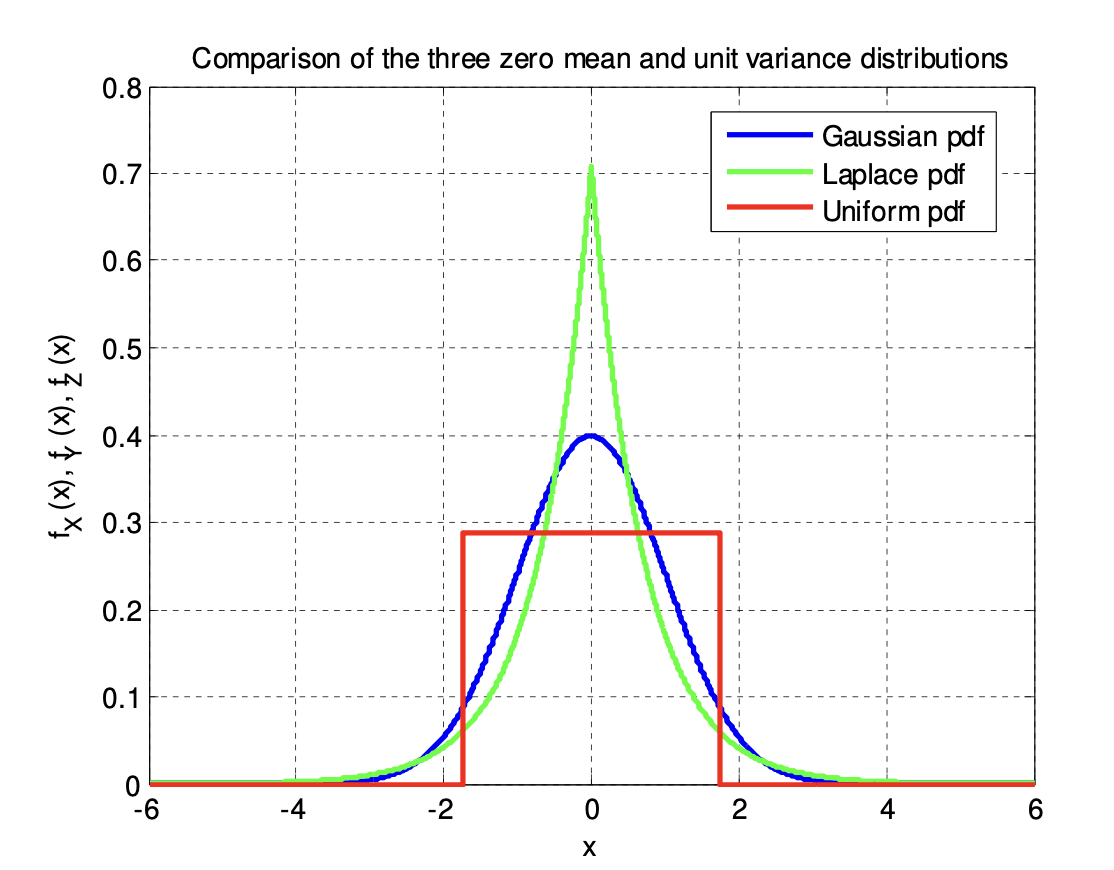
\includegraphics[width=0.6\linewidth]{Image/pdf 3/12.Comp_three.png}
    \label{fig:placeholder}
\end{figure}
\begin{figure}[H]
    \centering
    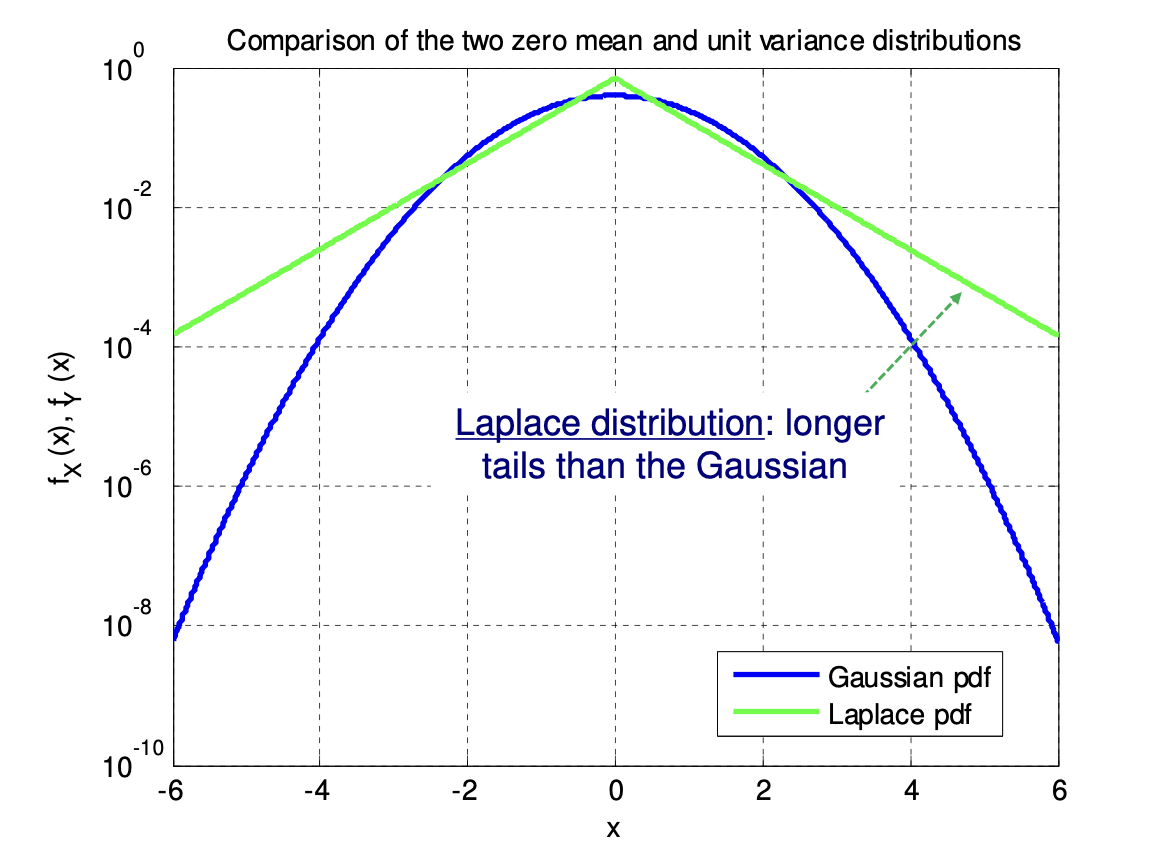
\includegraphics[width=0.6\linewidth]{Image/pdf 3/13.Comp_three_2.0.png}
    \label{fig:placeholder}
\end{figure}
\begin{figure}{H}
    \centering
    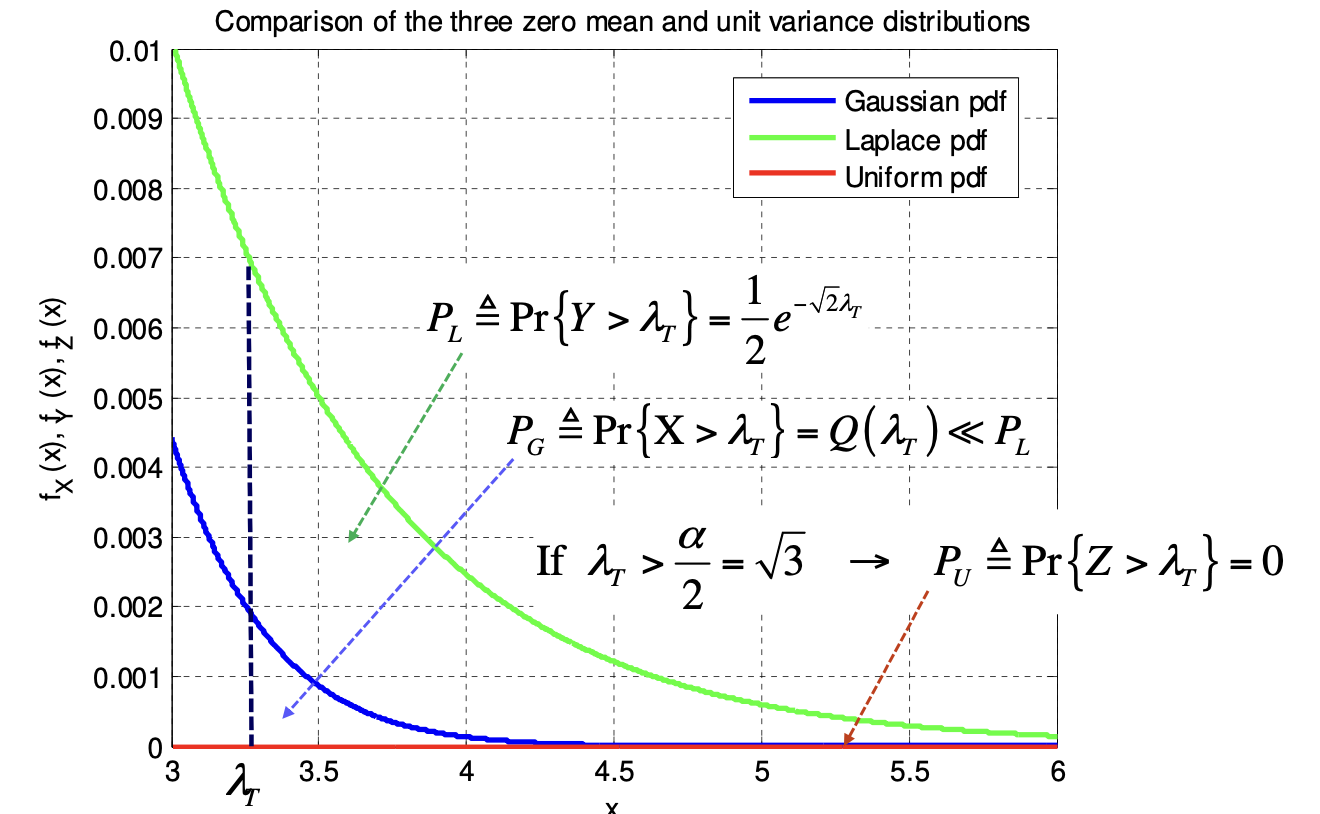
\includegraphics[width=0.6\linewidth]{Image/pdf 3/14.Comp_three_3.0.png}
    \label{fig:placeholder}
\end{figure}
\begin{figure}[H]
    \centering
    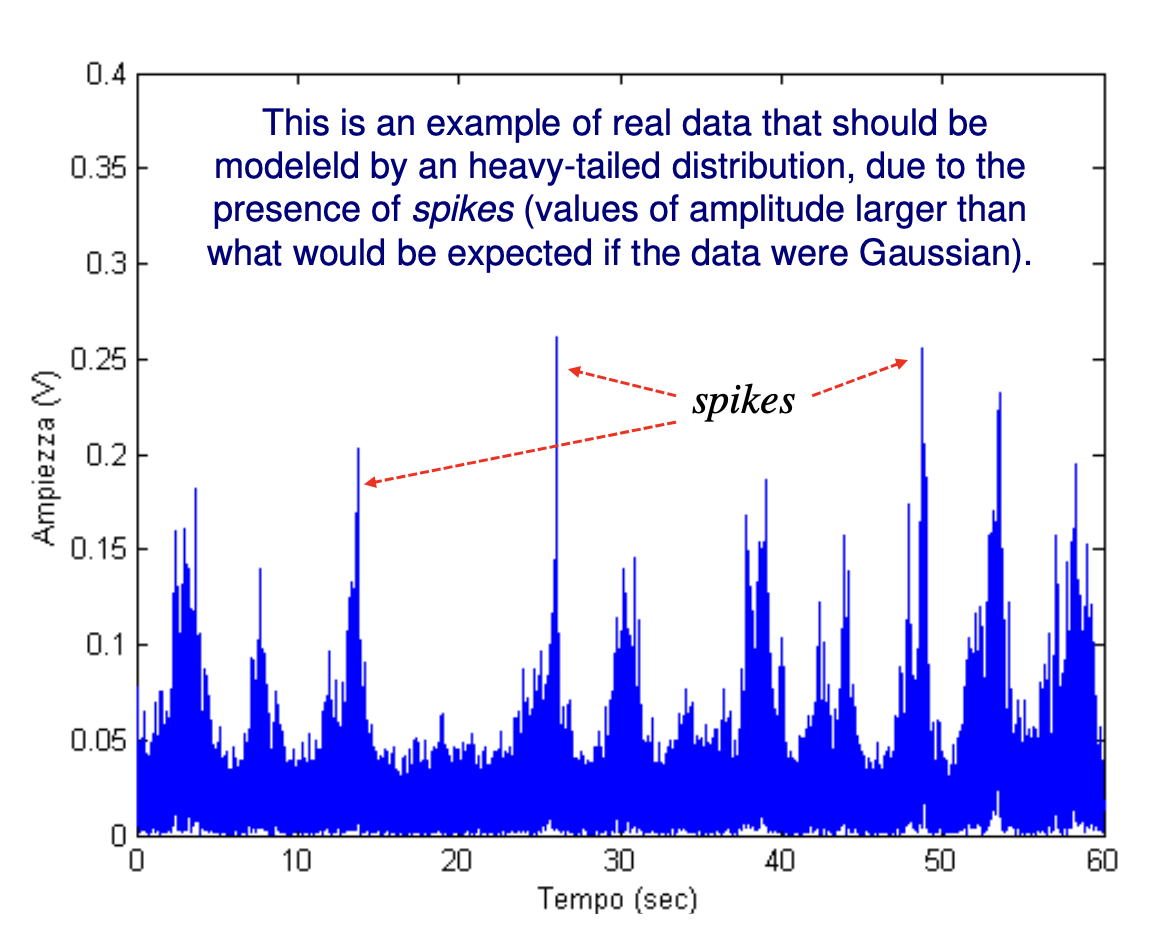
\includegraphics[width=0.6\linewidth]{Image/pdf 3/15.Comp_three_4.0.png}
    \label{fig:placeholder}
\end{figure}

\item \underline{In summary}, we can decide which pdf model to adopt for our observed data, based on the estimate of the first few moments, e.g. the first four as follows:
\begin{itemize}
    \item \textbf{Mean value:}
    \[
    \eta_X\triangleq E\{X\}\quad\Rightarrow\quad\hat{\eta}_X=\frac{1}{N}\sum_{i=1}^{N}X_i
    \]
    \item \textbf{Variance}:
\[
\sigma_X^2 \triangleq \mu_X(2) = E \left\{ (X - \eta_X)^2 \right\}
\implies
\hat{\sigma}_X^2 = \frac{1}{N} \sum_{i=1}^{N} (X_i - \hat{\eta}_X)^2
\]
    \item \textbf{Skewness}:
\[
\gamma_{3X} \triangleq \frac{\mu_X(3)}{\left(\mu_X(2)\right)^{3/2}}
= \frac{E\left\{ (X-\eta_X)^3 \right\}}{\left(E\left\{ (X-\eta_X)^2 \right\}\right)^{3/2}}
\implies
\hat{\gamma}_{3X} = \frac{\frac{1}{N} \sum_{i=1}^N (X_i - \hat{\eta}_X)^3}{\left(\hat{\sigma}_X^2\right)^{3/2}}
\]
    \item \textbf{Kurtosis}:
\[
\gamma_{4X} \triangleq \frac{\mu_X(4)}{(\mu_X(2))^2}-3
= \frac{E\left\{(X-\eta_X)^4\right\}}{(\mu_X(2))^2}-3
\implies
\hat{\gamma}_{4X}
= \frac{\frac{1}{N}\sum_{i=1}^N (X_i-\hat{\eta}_X)^4}{(\hat{\sigma}_X^2)^2}-3
\]   
\end{itemize}
\begin{figure}[H]
    \centering
    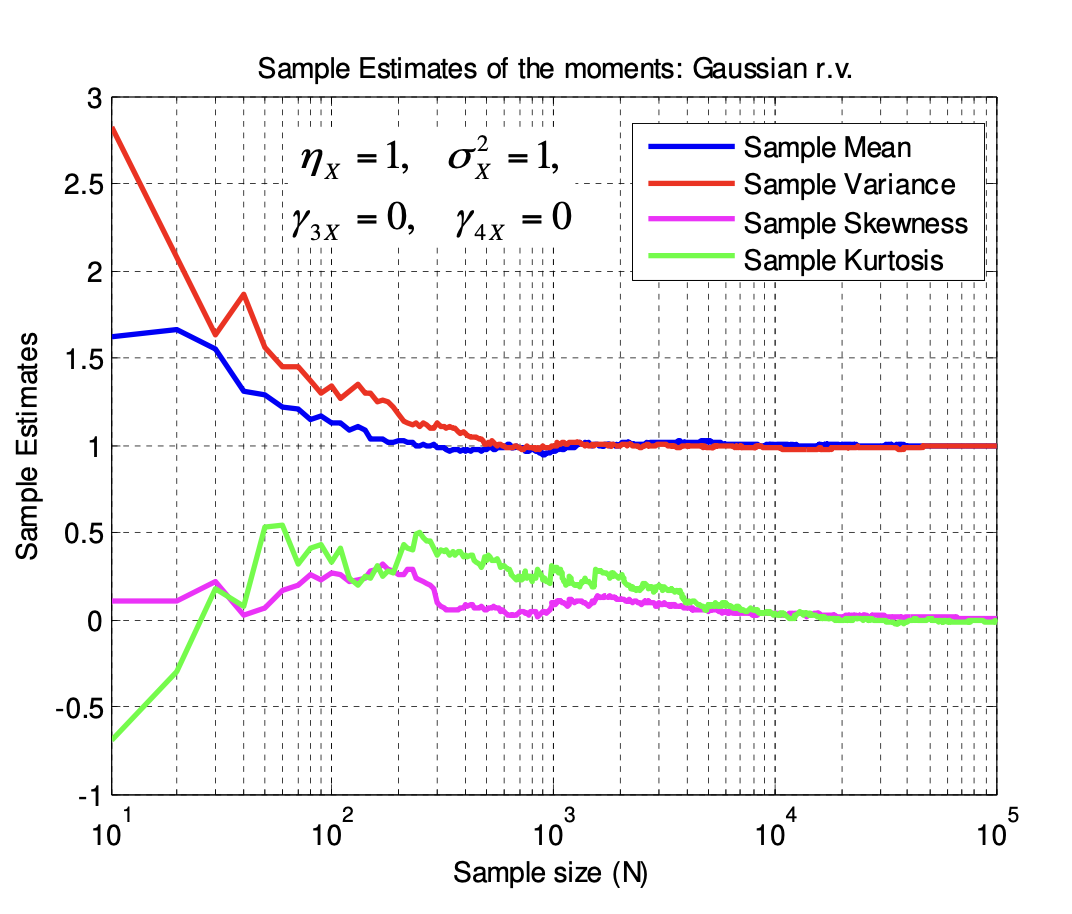
\includegraphics[width=0.55\linewidth]{Image/pdf 3/16.Sample_estimates.png}
    \label{fig:placeholder}
\end{figure}
\begin{figure}[H]
    \centering
    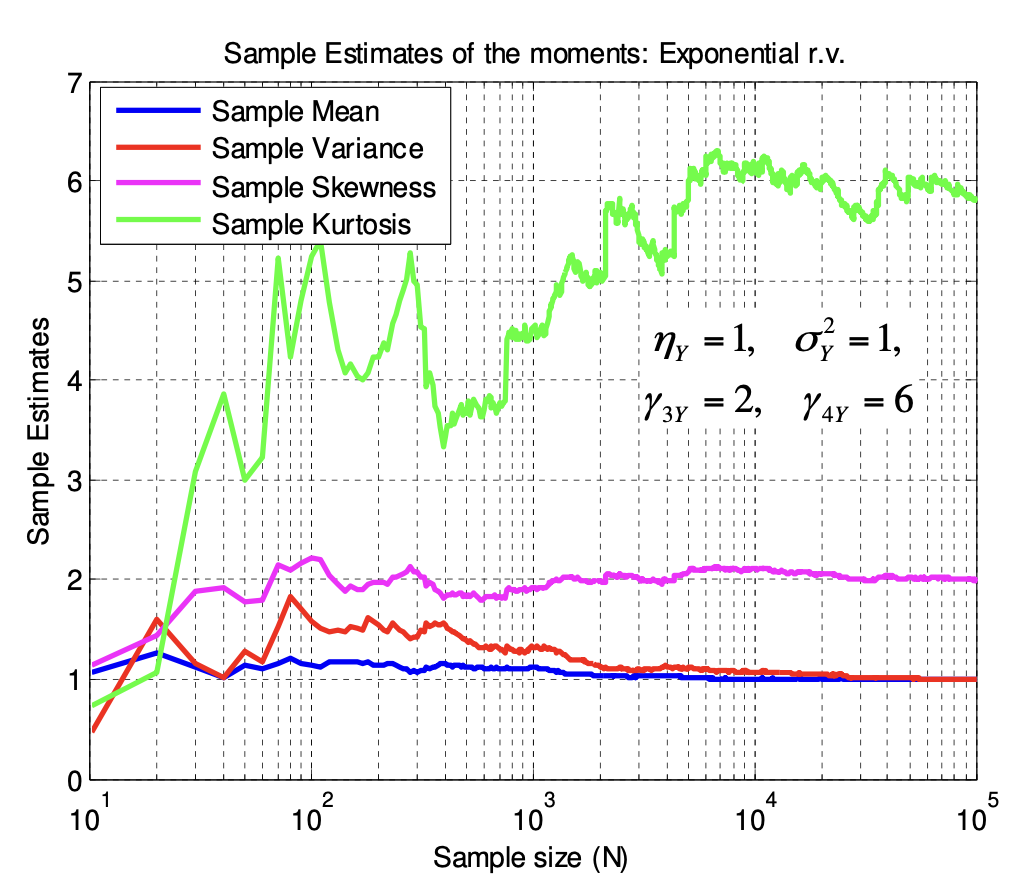
\includegraphics[width=0.6\linewidth]{Image/pdf 3/17.Sample_estimates_2.0.png}
    \label{fig:placeholder}
\end{figure}
\end{itemize}
\subsubsection{Measure of the Correlation Coefficient of 2 R.V's}
\begin{itemize}
    \item The same approach can be applied to estimate the \textbf{correlation coefficient} between two random variable \(X\) and \(Y\), if we can observe \(N\) independent realizations of \(X\) and \(Y\), i.e. we can collect \(N\) couples \(\{X_i,Y_i\}\):
\end{itemize}
\begin{figure}[H]
    \centering
    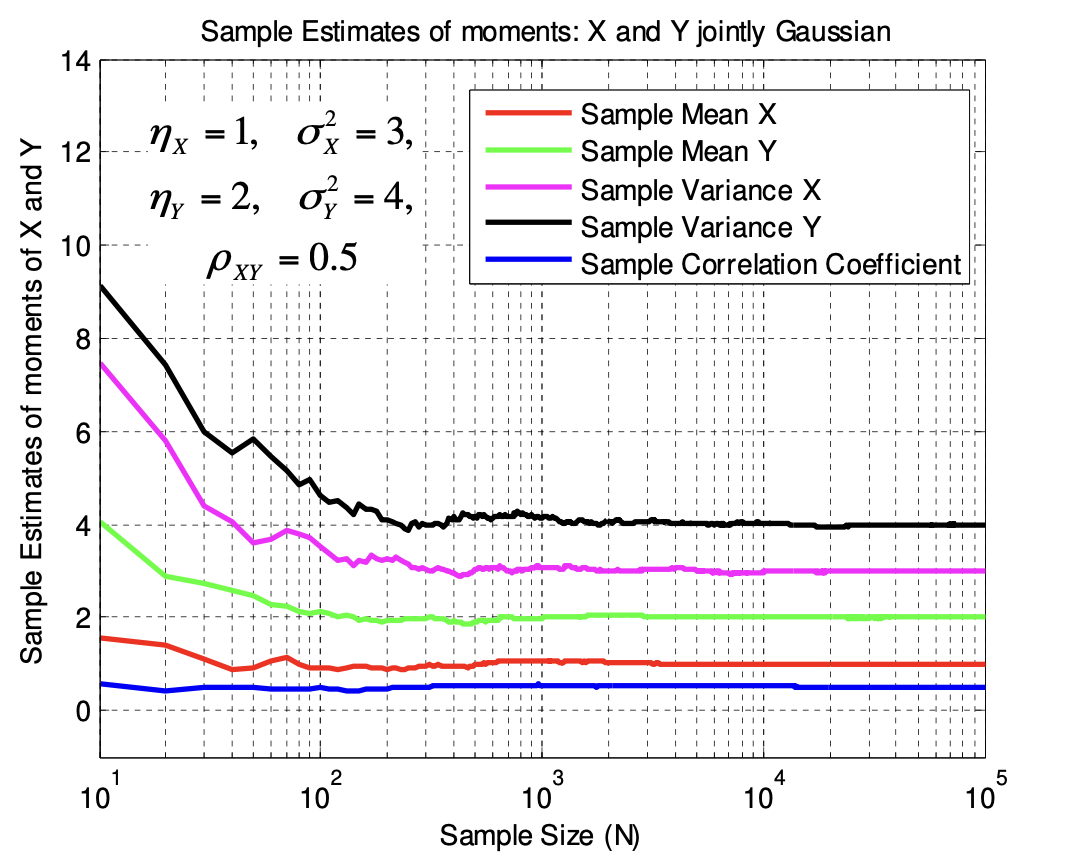
\includegraphics[width=0.6\linewidth]{Image/pdf 3/18.sample_estimates_corr.png}
    \label{fig:placeholder}
\end{figure}

\begin{figure}[H]
    \centering
    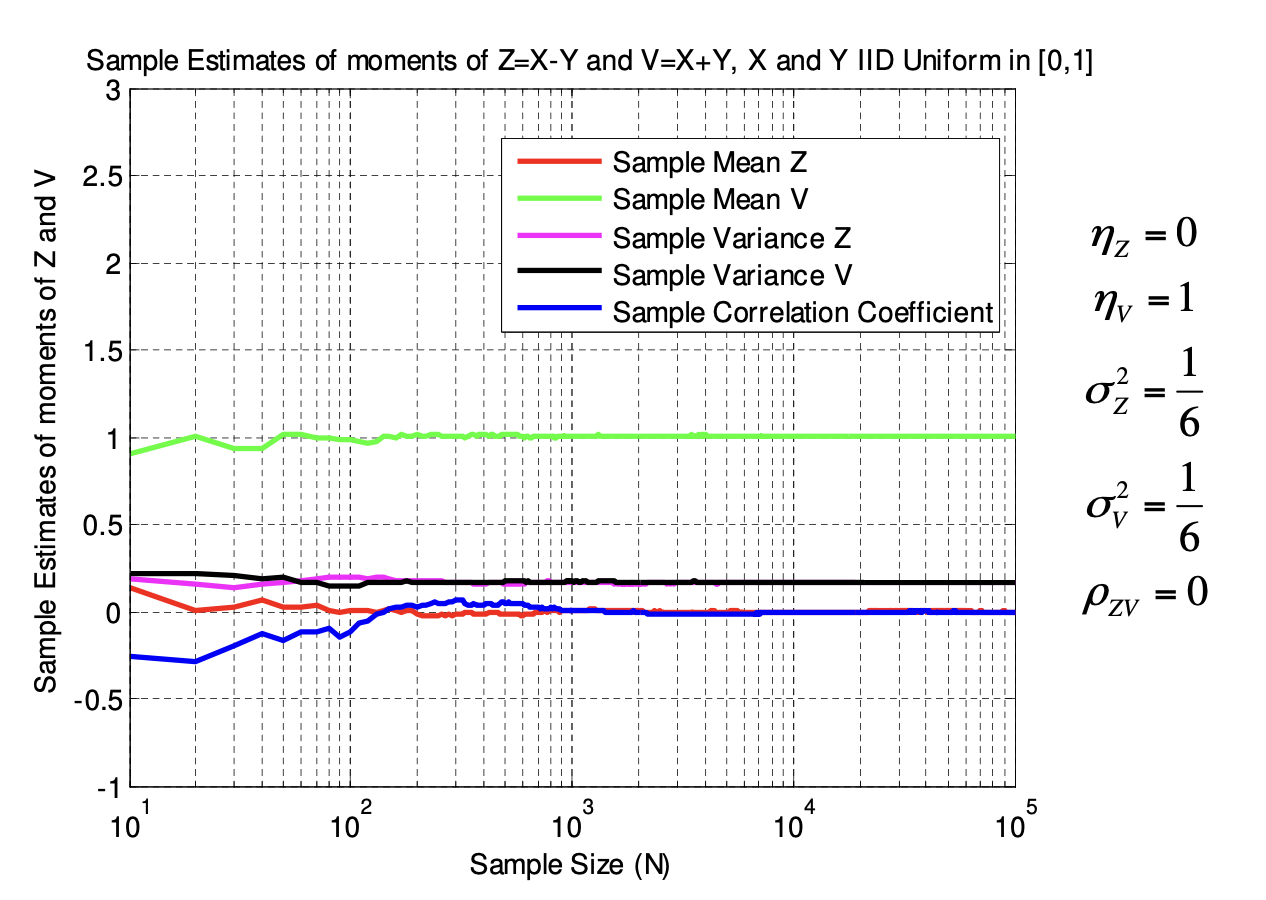
\includegraphics[width=0.6\linewidth]{Image/pdf 3/19.Sample_estimates_Corr_2.0.png}
    \label{fig:placeholder}

 
\end{figure}




(skip confidence interval)


\subsection{Measure of the Mean Value and of the Autocorrelation Function of a w.s.s Random Process}
\begin{itemize}
    \item Assume \(X[n]\) is wide sense stationary (w.s.s) process, how can we estimate the mean value and the autocorrelation function given \(N\) samples of the process:
    \(\{x[0],x[1],\cdots,x[N-1]\}\)
    \item Let's start from the mean value. We can apply the \textbf{Sample Mean estimator}:
\[
\eta_X \triangleq E \left\{ X[n] \right\}
\implies
\hat{\eta}_X = \frac{1}{N} \sum_{n=0}^{N-1} x[n]
\]
    \item The estimator is unbiased, in fact:
\[
b\{\hat{\eta}_X\} = E\{\eta_X - \hat{\eta}_X\} 
= \eta_X - \frac{1}{N}\sum_{n=0}^{N-1} E\{X[n]\} 
= \eta_X - \frac{1}{N}\sum_{n=0}^{N-1} \eta_X = 0
\]
    then the MSE and the variance coincide.

    \item The variance can be derived as follows:
\[
\begin{aligned}
\sigma_\varepsilon^2 &= \mathrm{var}\{\hat{\eta}_X\} = MSE\{\hat{\eta}_X\} = E\{(\eta_X - \hat{\eta}_X)^2\} \\
&= E\left\{ \left( \eta_X - \frac{1}{N} \sum_{n=0}^{N-1} X[n] \right)^2 \right\} 
= E\left\{ \left( \frac{1}{N} \sum_{n=0}^{N-1} \eta_X - \frac{1}{N} \sum_{n=0}^{N-1} X[n] \right)^2 \right\} \\
&= \frac{1}{N^2} E\left\{ \left( \sum_{n=0}^{N-1} (\eta_X - X[n]) \right)^2 \right\} 
= \frac{1}{N^2} E\left\{ \sum_{n=0}^{N-1} (\eta_X - X[n]) \sum_{k=0}^{N-1} (\eta_X - X[k]) \right\} \\
&= \frac{1}{N^2} E\left\{ \sum_{n=0}^{N-1} \sum_{k=0}^{N-1} (\eta_X - X[k]) (\eta_X - X[n]) \right\}
\end{aligned}
\]
\[
\begin{aligned}
\sigma_\varepsilon^2 
&= \frac{1}{N^2} E\left\{ \sum_{n=0}^{N-1} \sum_{k=0}^{N-1} (\eta_X - X[k]) (\eta_X - X[n]) \right\} 
= \frac{1}{N^2} \sum_{n=0}^{N-1} \sum_{k=0}^{N-1} E \left\{ (\eta_X - X[k]) (\eta_X - X[n]) \right\} \\
&= \frac{1}{N^2} \sum_{n=0}^{N-1} \sum_{k=0}^{N-1} C_X[n-k] 
=(*) \frac{1}{N^2} \sum_{m=-(N-1)}^{N-1} (N - |m|) C_X[m] \\
&= \frac{1}{N} \sum_{m=-(N-1)}^{N-1} \left( 1 - \frac{|m|}{N} \right) C_X[m]
\end{aligned}
\]
\begin{itemize}
    \item \(C_X[m]\) is the \textbf{Auto-Covariance function of the process}.
    \item \(\left(1-\frac{|m|}{N}\right)\) is a \textbf{Triangular weighting window}.
    \item \(*\) we used the \textbf{"Double sum"} formula:
    
\[
\sum_{n=0}^{N-1} \sum_{k=0}^{N-1} f[n-k] 
= \sum_{m=-(N-1)}^{N-1} (N - |m|) f[m]
\]
\end{itemize} 
\item The \textbf{necessary and sufficient condition} in order the \textbf{sample mean} to be a \textbf{consistent} estimator of the statistical mean of the process is :


\item If the process has finite memory, that is \(C_X[m]\) has a strictly limited length (e.g. the MA processes), or goes to zero "relatively" fast (e.g. for the stable AR or ARMA processes) then the estimator is consistent, i.e. its MSE goes to zero when the number of data \(N\) goes to infinity.\\
When does this happen? \textbf{The independence assumption is not necessary}

\item \textbf{Example 1}: \(X[n]\) is an autoregressive process of order 1, AR(1):
\[
\begin{aligned}
C_X[m] 
&= R_X[m] = E\{X[n]X[n+m]\} = \sigma_X^2 \rho^{|m|}, \quad \text{where } |\rho| < 1
\\[1ex]
MSE\{\hat{\eta}_X\} 
&= \frac{1}{N^2} \sum_{n=0}^{N-1} \sum_{k=0}^{N-1} C_X[n-k] = \frac{1}{N^2} \sum_{n=0}^{N-1} \sum_{k=0}^{N-1} \sigma_X^2 \rho^{|n-k|}\\[1ex]
&= \frac{\sigma_X^2}{N^2} \sum_{m=-(N-1)}^{N-1} (N-|m|) |\rho|^{|m|}
\leq \frac{\sigma_X^2}{N^2} \sum_{m=-(N-1)}^{N-1} N |\rho|^{|m|}
\\[1ex]
&= \frac{\sigma_X^2}{N} \sum_{m=-(N-1)}^{N-1} |\rho|^{|m|}
= \frac{\sigma_X^2}{N} \left(2\sum_{m=0}^{N-1} |\rho|^m - 1\right)
= \frac{\sigma_X^2}{N} \left(2 \cdot \frac{1-|\rho|^N}{1-|\rho|} - 1\right)
\end{aligned}
\]

\noindent In this case, the \textbf{Sample Mean} is a consistent estimator
\[
\lim_{N \to \infty} MSE\{\hat{\eta}_X\}
= \lim_{N \to \infty} \left[ \frac{\sigma_X^2}{N} \left( \frac{1+|\rho|-2|\rho|^N}{1-|\rho|} \right) \right]
= 0, \quad \text{if } |\rho|\neq 1
\]
\noindent When \(\rho=0\), i.e. we go back to the case of independent data:
\[
MSE\{\hat{\eta}_X\}\Big|_{\rho=0}=\frac{\sigma_X^2}{N}
\]
\noindent Hence, \underline{the assumption of data independence is a sufficient condition for the Sample Mean}\\
\noindent\underline{to be consistent, but it is not a necessary condition}[Remember that instead the assumption that the data are identically distributed is necessary]

\item \textbf{Example 2}: observed data = constant signal + independent noise
\[
\begin{aligned}
& X[n] = S + W[n] \\[2ex]
& S \in \mathcal{N}(0, \sigma_S^2), \quad W[n] \in \mathcal{N}(0, \sigma_W^2), \quad \{W[n]\}_{n=0}^{N-1} \text{ IID}, \\[2ex]
& W[n] \text{ white noise, } S \text{ and } W[n] \text{ independent} \\[2ex]
& \eta_X[n] = E\{X[n]\} = E\{S + W[n]\} = 0 \\[2ex]
& \gamma \triangleq \frac{E\{S^2\}}{E\{W^2[n]\}} = \frac{\sigma_S^2}{\sigma_W^2} \quad [\text{SNR}]
\end{aligned}
\]
\noindent\textbf{Autocovariance function}:
\[
\begin{aligned}
C_X[m] = R_X[m] = E\{X[n] X[n+m]\} 
&= E\{ (S + W[n])(S + W[n+m]) \} 
\\[2ex]
&= E\{ S^2 + S W[n] + S W[n+m] + W[n]W[n+m] \}
\\[2ex]
&= E\{S^2\} + E\{W[n]W[n+m]\}
\\[2ex]
&= \sigma_S^2 + \sigma_W^2 \delta[m]
\end{aligned}
\]
\noindent\textbf{Variance}:
\[
\sigma_X^2=C_X[0]=\sigma_S^2+\sigma_W^2
\]
\noindent\textbf{Normalized autocovariance function}:
\[
\begin{aligned}
\rho_X[m] &\triangleq \frac{\text{cov} \{ X[n], X[n+m] \}}{\sqrt{\text{var}\{ X[n] \} \text{var}\{ X[n+m] \}}}
= \frac{C_X[m]}{C_X[0]} = \frac{\sigma_S^2 + \sigma_W^2 \delta[m]}{\sigma_X^2}
\\[2ex]
&= \frac{\sigma_S^2}{\sigma_S^2 + \sigma_W^2}
+ \frac{\sigma_W^2}{\sigma_S^2 + \sigma_W^2} \delta[m]
\\[2ex]
\forall m \neq 0 \quad &\Rightarrow \quad \rho \triangleq \rho_X[m] = \frac{\sigma_S^2}{\sigma_S^2 + \sigma_W^2} = \frac{\gamma}{\gamma + 1}
\\[2ex]
\forall m \neq 0 \quad &\Rightarrow \quad C_X[m] = \rho (\sigma_S^2 + \sigma_W^2) = \rho \sigma_X^2
\end{aligned}
\]
\noindent\(\rho\) is the correlation coefficient between \(X[n]\) and \(X[n+m]\).\\
\noindent Hence, in this case we get:
\[
\begin{aligned}
MSE\{\hat{\eta}_X\}
&= \frac{1}{N^2} \sum_{n=0}^{N-1}\sum_{k=0}^{N-1} C_X[n-k]
= \frac{C_X[0]}{N} + \frac{1}{N^2} \sum_{\substack{n=1 \\ n\neq k}}^{N-1}\sum_{k=1}^{N-1} C_X[n-k]
\\[2ex]
&= \frac{\sigma_X^2}{N} + \frac{1}{N^2} \sum_{n=1}^{N-1}\sum_{k=1}^{N-1} \rho \sigma_X^2
= \frac{\sigma_X^2}{N} + \frac{N(N-1)}{N^2} \rho \sigma_X^2
\\[2ex]
&= \frac{\sigma_X^2}{N} + \rho \sigma_X^2 \left(1-\frac{1}{N}\right)
\\[2ex]
\lim_{N\to\infty} MSE\{\hat{\eta}_X\} 
&= \lim_{N\to\infty} \left[ \frac{\sigma_X^2}{N} + \rho \sigma_X^2 \left(1-\frac{1}{N}\right) \right]
= \rho \sigma_X^2 = \sigma_S^2 \ne 0 \quad \text{if } \rho \ne 0
\end{aligned}
\]
\noindent In this case, the \textbf{Sample Mean} is \textbf{not} a consistent estimator of the mean \(\eta_X\).


\item \textbf{Important}: If the samples \(X[n]\) are uncorrelated, then :
\[
C_X[m] = \sigma_X^2 \delta[m]
\implies
\sigma_\varepsilon^2 = \frac{1}{N} \sum_{m=-(N-1)}^{N-1} \left(1-\frac{|m|}{N}\right) \sigma_X^2 \delta[m]
= \frac{\sigma_X^2}{N}
\]
\noindent so the MSE decreases as \(1/N\).

\item Note that if the data are (positively) correlated, then the MSE is larger.

\item \textbf{Estimate of the Autocorrelation function(ACF)}, given \(N\) samples of the process: \(\{x[0],x[1],\cdots,x[N-1]\}\).
\item Again, we can apply the \textbf{Sample Estimators}:

\[
R_X[m] \triangleq E\left\{ X[n] X^*[n+m] \right\}
\implies
\hat{R}_X[m] = \frac{1}{N} \sum_{n=0}^{N-1} x[n]\, x^*[n+m]
\]
\item Note that, since we collect data only from discrete-time \(0\) to \(N-1\), the maximum value for \(n+m\) is \(N-1\), so the estimator should be expressed as:
\[
\tilde{R}_X[m] = \frac{1}{N-m} \sum_{n=0}^{N-m-1} x[n]\, x^*[n+m],\quad m = 0, 1, 2,\,\dots,\, N-1
\]
\item Where \(N-m\) is the number of products that we average. This is called the (unbiased) \textbf{Sample Autocorrelation Function}.
\item The estimate for negative values of \(m\) are obtained by resorting to the Hermitian symmetry property of the ACF:
\[
\tilde{R}_X[m] = \tilde{R}_X^*[-m],\quad m = -1, -2,\, \dots,\, -(N-1)
\]
\item This estimator is called the \textbf{unbiased Sample ACF}, since it is unbiased for lags \(m=0,1,2,\cdots,N-1\):
\[
\begin{aligned}
E\left\{ \tilde{R}_X[m] \right\}
&= \frac{1}{N-m} \sum_{n=0}^{N-m-1} E\left\{ X[n] X^*[n+m] \right\}
\\[2ex]
&= \frac{1}{N-m} \sum_{n=0}^{N-m-1} R_X[m] = R_X[m], \quad \text{for } 0 \leq m \leq N-1
\end{aligned}
\]
\item Hence, for \(|m|<N\), the error mean value is zero; this justifies the epithet unbiased estimate, somehow.
\item The main drawback of this estimator is the fact that, as \(m\) increases, the number of products \(X[n]X^*[n+m]\)) decreases, since it is equal to \(N-m\). Consequently, the error variances increases with \(m\).
\item The worst case is when \(m=N-1\): in this case \(N-m=1\), so only  a single product can be evaluated \(\rightarrow\) there is no averaging at all. The product \(X[N-1]X^*[0]\) can assume very large values, depending on the power of the process, even if \(R_X[N-1]\) is very small or equal to zero, then the estimation error can be very large.
\item Typically, for processes that do not contain periodic components, the ACF tends to 0 when \(m\) increases (with a convergence speed that depends on the bandwidth of the process). To take this into account, the sample estimator can be modified as follows:

\item This is called the \textbf{biased Sample ACF} and it has generally a smaller error than the unbiased one as \(m\) tends to \(N-1\), since the unbiased estimate can assume large values for \(m\) close to \(N-1\).
\item For small values of \(m\) the biased and the unbiased estimators have similar performance, since \(N-m\approx N\).
\item The bias of the \textbf{biased Sample ACF} can be easily derived:
\[
\begin{aligned}
\hat{R}_X[m] &= \left( \frac{N-m}{N} \right) \tilde{R}_X[m] = \left(1-\frac{m}{N}\right) \tilde{R}_X[m], \quad \text{for } 0 \leq m \leq N-1
\\[2ex]
E\left\{ \hat{R}_X[m] \right\} &= \left(1-\frac{m}{N}\right) E\left\{ \tilde{R}_X[m] \right\} = \left(1-\frac{m}{N}\right) R_X[m]
\\[2ex]
b\left\{ \hat{R}_X[m] \right\} &= \frac{m}{N} R_X[m], \quad \text{for } 0 \leq m \leq N-1
\end{aligned}
\]
\item The bias tends to increase linearly with \(m\), but if the ACF does not contain periodic components, it typically tends to 0 in such a way that the bias tends to 0.

\item \textbf{MSE of the biased Sample ACF vs the MSE of the unbiased Sample ACF}:
\[
\begin{aligned}
\hat{R}_X[m] &= \left(1-\frac{m}{N}\right) \tilde{R}_X[m], \quad \text{for } 0 \leq m \leq N-1
\\[2ex]
MSE\left\{\hat{R}_X[m]\right\} 
&= \left( b\{\hat{R}_X[m]\} \right)^2 + \mathrm{var}\left\{\hat{R}_X[m]\right\}
\\
&= \left( \frac{m}{N} R_X[m] \right)^2 + \left(1-\frac{m}{N}\right)^2 \mathrm{var}\left\{\tilde{R}_X[m]\right\}
\\
&= \left( \frac{m}{N} R_X[m] \right)^2 + \left(1-\frac{m}{N}\right)^2 MSE\left\{ \tilde{R}_X[m] \right\}, \quad \text{for } 0 \leq m \leq N-1
\end{aligned}
\]
\item The presence of a bias makes the MSE of the biased Sample ACF estimator to increase, but the reduction in variance is such that overall its MSE generally decreases (again, if the ACF does not contain periodic components).

\item The \textbf{biased Sample ACF} always provides a positive definite estimate, i.e.
its Fourier transform is always positive. Instead, the FT of the \textbf{unbiased Sample ACF} could be negative for some values of the frequency. This can be a problem since the PSD, that is the FT of the ACF, should always be positive.
\item Let us see some numerical results for a \textbf{Markov process}, i.e. an AR(1) process:
\[
R_X[m] \triangleq E\left\{ X[n] X[n+m] \right\}
= \sigma_X^2 \rho^{|m|}, \quad |\rho| < 1
\]
\item Assume: \(\sigma_X^2=1\)

\begin{figure}[H]
    \centering
    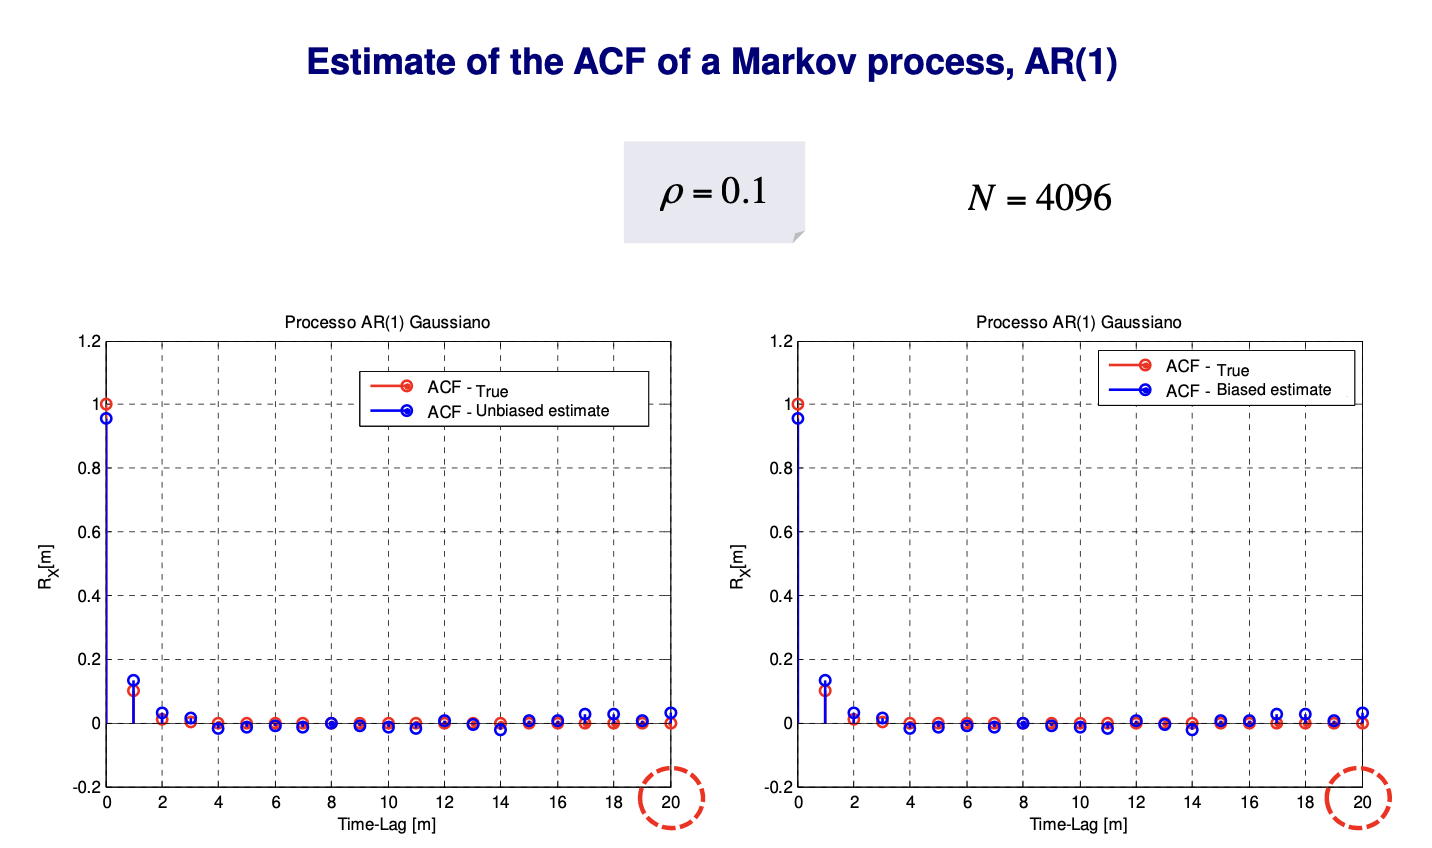
\includegraphics[width=0.6\linewidth]{Image/pdf 3/20.Estimate_of_the ACF_markov_Process.png}

    \label{fig:placeholder}
\end{figure}
\begin{figure}[H]
    \centering
    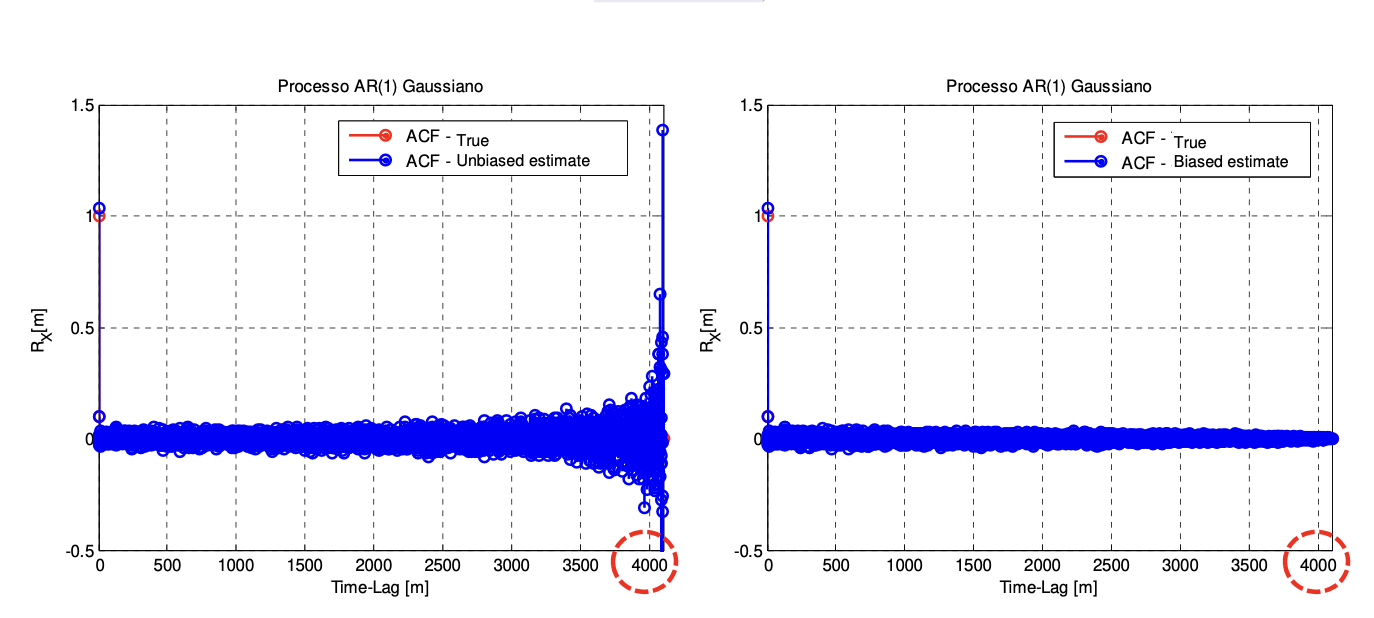
\includegraphics[width=0.6\linewidth]{Image/pdf 3/21.estimate_2.0.png}
    \label{fig:placeholder}
\end{figure}
\begin{figure}[H]
    \centering
    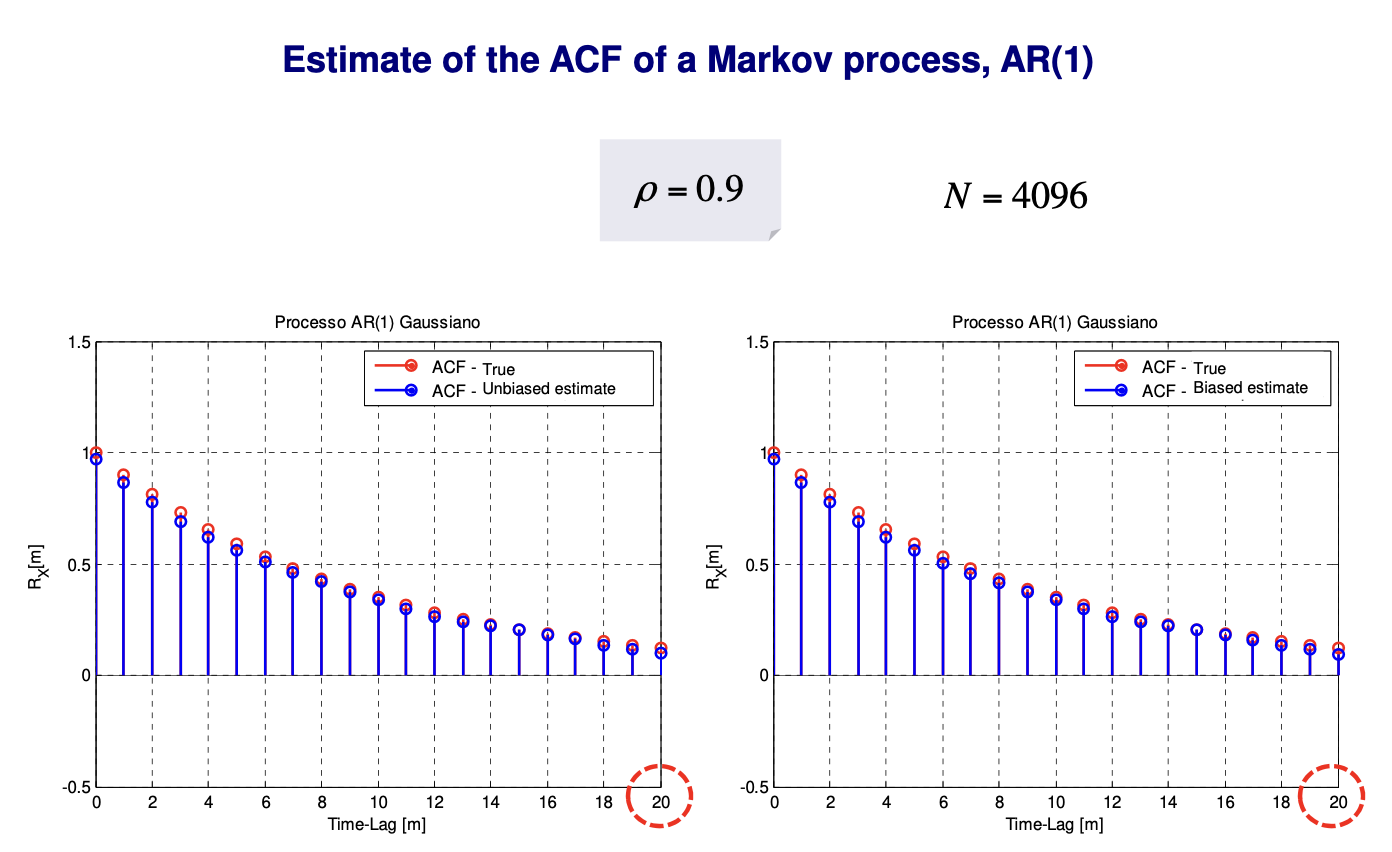
\includegraphics[width=0.6\linewidth]{Image/pdf 3/22.3.0.png}
    \label{fig:placeholder}
\end{figure}
\begin{figure}[H]
    \centering
    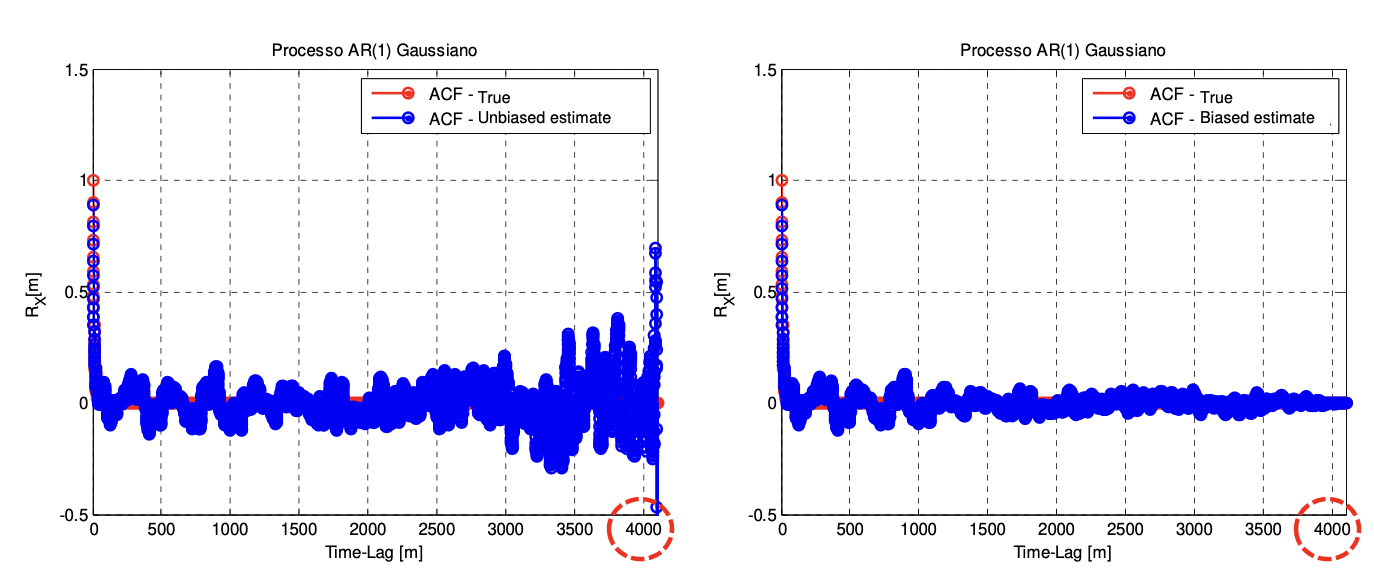
\includegraphics[width=0.6\linewidth]{Image/pdf 3/23.4.0.png}
    \label{fig:placeholder}
\end{figure}



\end{itemize}


\clearpage


